\documentclass[11pt]{article}
\usepackage[letterpaper,margin=1in]{geometry}
\usepackage{amsmath,amssymb,amsthm}
\usepackage{booktabs}
\usepackage{graphicx}
\usepackage[colorlinks=true,linkcolor=blue,citecolor=blue,urlcolor=blue]{hyperref}
\newtheorem{theorem}{Theorem}
\newtheorem{proposition}[theorem]{Proposition}
\newtheorem{corollary}[theorem]{Corollary}
\newtheorem{lemma}[theorem]{Lemma}
\newtheorem{remark}[theorem]{Remark}
\newcommand{\TV}{\mathrm{TV}}
\newcommand{\KL}{D_{\mathrm{KL}}}
\newcommand{\E}{\mathbb{E}}
\newcommand{\todo}[1]{\textcolor{red}{[TODO: #1]}}
\usepackage{xcolor}

\title{\textbf{The Value of Delayed Information:\\
Predictive-Information Envelopes for Age-Limited Decisions}\\[4pt]
\large Envelopes, exact laws, and witnesses for age-limited decisions}
\author{Andrew H. Bond,~\emph{Senior Member, IEEE}\\
Department of Computer Engineering, San Jos\'e State University\\
\texttt{andrew.bond@sjsu.edu} ~\textbar~ ORCID: 0009-0003-2599-6158}
\date{Working draft --- v1.0 (submission candidate: max-statistic target stated correctly; selection-aware column in Table 2)}

\setlength{\emergencystretch}{2em}
\usepackage{placeins}
\begin{document}
\maketitle

\begin{abstract}
A controller that acts on delayed information, through a sensing lag, a
telemetry delay or a stale cache, can beat the best static policy only
insofar as the delayed observation still predicts the current state. A
companion systems submission \cite{infocom} proves this exactly for
symmetric two-state Markov capacity. This paper supplies the general
theory. It isolates the exact quantity, the Bayes envelope, which is the
expected excess value of posterior over prior beliefs, and restates in
value-of-information form an envelope known from the minimum-excess-risk
literature that bounds it by the square root of the mutual information
between the delayed observation and the current state. Three consequences
follow. An observation carrying a fixed number of bits caps the value of
feedback whatever it encodes. The envelope is tight to leading order for
the symmetric binary chain. No universal formula can map mutual
information to decision value, because two observations with identical
information can carry all or none of the decision-relevant distinction.
For binary state, the local decision geometry at the prior sets how value
grows with correlation: as a sum of hinges with dead zones for finite
action sets, and quadratically when the value function is smooth. A
ten-series battery across acoustics, bioacoustics, space weather,
seismology and the BGP control plane of the Internet, with synthetic
controls, tests these predictions. Two series, a teleseismic earthquake
record and a BGP update stream, carry material history value, and
calendar blocks show that the value is concentrated in identifiable regimes. A
chain-rule decomposition separates what history reveals about the regime
from what it predicts within one, and the envelope inverts into
dependence-aware lower bounds on conditional predictive information. All
history values are measured for a protocol-fixed six-lag lookup policy and are
lower bounds on what a richer policy could extract. When actions move the
state, the envelope still bounds the decision value of delayed
information under the law the controller induces, but not the value of
steering, and in a registered closed-loop queue almost all of the feedback
gain is steering.
\end{abstract}

\section{Introduction}\label{sec:intro}

Everywhere a controller acts on stale state (a scheduler admitting jobs
against capacity sensed seconds ago, a trader on delayed quotes, a relay on
an outdated channel estimate), the same question recurs: \emph{what is the
value of information of age $D$?} The age-of-information literature
\cite{yates21} measures freshness; freshness, however, has no decision
semantics: a maximally fresh sample of an i.i.d.\ process is worthless, and
a stale sample of a slowly-mixing one is nearly as good as the present. Our
companion systems paper \cite{infocom} made this precise in one setting,
proving that for symmetric two-state Markov capacity the advantage of
age-$D$ feedback over the best static policy is \emph{exactly}
$\Delta(D)=\tfrac12 r(D)$ (with $r(D)$ the autocorrelation at the sensing lag), and
measuring the law on a live GPU cluster. This paper supplies the theory that
result belongs to. The thesis is one line:
\begin{center}\emph{Age matters only through predictive information, and
predictive information matters only through the Bayes envelope.}\end{center}

Concretely: (\textbf{C1}) we isolate the exact object, the Bayes envelope
$\Delta_Y=\E[\psi(\mu_Y)]-\psi(\bar\mu)$, classical in decision theory
\cite{howard1966,raiffa61,delaragossner}, and restate in that frame the
\emph{predictive-information envelope}
$\Delta_Y\le\Omega\sqrt{I(X;Y)/2}$ (Theorem~\ref{thm:mi}; known as a
minimum-excess-risk inequality, attribution in \S\ref{sec:mi}), with the
\emph{bit-budget corollary}: an observation carrying at most $b$ bits
($H(Y)\le b\ln 2$) caps feedback value at $\Omega\sqrt{(b\ln2)/2}$, so
compression can preserve but never create feedback value. For integer $b$, the cap
improves on the trivial range bound only when $b\le2$, and a controller that accumulates messages across decisions
holds a richer observation to which the corollary applies with its total
entropy. (\textbf{C2}) We show the envelope is \emph{sharp
where it matters}: on the canonical binary chain it matches the exact law to
$O(r^3)$ (Proposition~\ref{prop:tight}), and the battery of
\S\ref{sec:battery} \emph{illustrates} this tightness on real binary
pair distributions (a
consistency check: $\hat I$ and $\widehat V_1$ derive
from the same lag table). (\textbf{C3}) We prove no universal
equality $\Delta=f(I)$ exists for bounded objectives
(Proposition~\ref{prop:noneq}): information is a scalar, value is a
geometry. This stands in contrast to the classical exception. For
\emph{logarithmic} (unbounded) utility, Kelly and Barron--Cover
\cite{kelly56,barroncover88} show the value of side information \emph{equals}
$I$. For general bounded objectives, mutual information provides a
universal envelope but does not determine value; logarithmic utility is a
distinguished objective for which equality is possible.
(\textbf{C4}) We give an exactness theory for binary state whose organizing
fact is that \emph{the local geometry of the value function at the prior
sets the correlation exponent}. For finite action sets (polyhedral value
functions) the value of a delayed sample is exactly a sum of
\emph{hinges} in the lag-$D$ covariance, with sign-dependent dead-zone
thresholds (linear response beyond, identically zero within); when the
value function $\psi$ is twice differentiable at the prior with
$\psi''>0$, the weak-correlation response is quadratic to leading order
(exactly $C(D)^2/\pi(1-\pi)$ for squared error); and a prior sitting on
a kink (the companion's symmetric case) is the polyhedral
configuration yielding threshold-free linear response
(\S\ref{sec:multistate}). The dead zone is the sharp polyhedral form of the
Radner--Stiglitz nonconcavity of the value of information
\cite{radnerstiglitz84,chadeschlee02}: when the prior sits off a kink of a polyhedral
objective, weakly-correlated feedback is \emph{worthless}, not merely weak,
and the sign of the correlation matters. (\textbf{C5}) We order the three
envelopes (mixing, information, bit-budget) below the master
total-variation envelope and prove mixing and information are incomparable.
For every lag and every $K$, a \emph{preview process} keeps
$\beta(D)\ge\tfrac12$ while the information envelope, and the true value,
vanish with $K$ (\S\ref{sec:comparison}). (\textbf{C6}) Across ten
series from four physical domains, one computer system and controls, the
battery establishes equivalence for the protocol-fixed policy class on
three series, leaves one noise-limited and one inconclusive, records two
smaller detections near the practical threshold, and finds material
history gains on two, a teleseismic record and a BGP update stream; the
i.i.d.\ series serves as the selection control. Calendar blocks show both gains
concentrated in identifiable regimes, which a chain-rule decomposition
(Lemma~\ref{lem:regime}) separates into regime identification and
within-regime prediction. Read backwards, the incremental theorem
converts each gain into a model-calibrated, dependence-aware lower bound
on \emph{conditional} history information, always one-sided:
$I(X_t;\text{history}\mid X_{t-D})\ge
2[(\widehat\Delta_W-\widehat\Delta_Z-\varepsilon)^{+}]^2$
(\S\ref{sec:battery}). Every history value in the battery is measured for
a protocol-fixed six-lag lookup policy, so it is a lower bound on what a
richer policy (longer lags, a recurrent model) could extract, and every
negative finding is a statement about that policy class. (\textbf{C7}) We
close the loop: the envelope survives any closed-loop controller as a
bound on decision value under the law that controller induces
(Proposition~\ref{prop:clstep}), steering value has no information envelope
(Proposition~\ref{prop:clsteer}, machine-checked for every horizon), and a
registered closed-loop queue attributes at least $99\%$ of its feedback gain
to steering (\S\ref{sec:queue}).

Table~\ref{tab:novelty} separates what this paper restates from what it adds. The
finite and algebraic results are machine-checked in Lean~4 against Mathlib
(73 theorems, including the closed-loop counterexample for every horizon),
and the analytic ones symbolically; both are part of the
released artifact.

\begin{table}[!ht]\centering\small
\begin{tabular}{p{0.58\linewidth}p{0.36\linewidth}}
\toprule
Component & Status \\
\midrule
Bayes envelope \eqref{eq:envelope} & classical \cite{howard1966,raiffa61,delaragossner} \\
Information envelopes (Thm.~\ref{thm:mi}, Thm.~\ref{thm:incr}) & known minimum-excess-risk inequalities, restated \\
Garbling monotonicity (Lemma~\ref{lem:blackwell}) & classical (Blackwell) \\
Bit-budget corollary (Cor.~\ref{cor:bits}) & immediate from $I(X;Y)\le H(Y)$ \\
No universal $\Delta=f(I)$ (Prop.~\ref{prop:noneq}) & elementary construction \\
Local marginal-value trichotomy & known \cite{delaragossner} \\
Exact lag-covariance hinge law, sign-asymmetric thresholds (Thm.~\ref{thm:hinge}) & new, to our knowledge \\
Explicit contact-order coefficients (Thm.~\ref{thm:contact}) & new, to our knowledge \\
Mixing/information separation construction (Prop.~\ref{prop:incomp}) & new, to our knowledge \\
Regime decomposition (Lemma~\ref{lem:regime}) & elementary (chain rule) \\
Closed loop: per-step envelope (Prop.~\ref{prop:clstep}) and the steering
counterexample (Prop.~\ref{prop:clsteer}) & new, to our knowledge \\
Conditional-information certificate from policy gain & new operational use \\
Multi-domain battery with a BGP series and regime analysis (\S\ref{sec:battery}) & new \\
\bottomrule
\end{tabular}
\caption{What is known and what is new. The known results are restated because the exact laws and the battery are built on them.}
\label{tab:novelty}
\end{table}

The scope is stated precisely: this is a unified theory for
\emph{exogenous one-step bounded-reward decisions} under delay. The
action does not move the state, and the reward is single-stage. Within that
scope the theory is closed on itself: one decision-theoretic object
explaining an exact systems law, envelopes ordered by what they require
(a model, samples, or a bit rate), sharpness results tying envelope to law,
impossibility results delimiting both, and a falsifiable empirical program
run on real processes from four physical domains and one computer system.
Section~\ref{sec:closedloop} says exactly what transfers when actions do move
the state: the envelope still bounds the decision value of delayed
information under whatever law a closed-loop controller induces, and it
does not bound the value of steering, which can grow without limit while
every per-step envelope stays small.

\section{Setting and the exact object}\label{sec:envelope}

Let $X$ be the current exogenous state taking values in a finite set
$\mathcal X$, with marginal $\bar\mu$. A controller observes a delayed
quantity $Y$ (a delayed sample $X_{t-D}$, a delayed history, or any
$\sigma(\mathcal F_{\le t-D})$-measurable statistic), chooses an action $w$,
and receives a bounded one-step reward $R(w,x)$ with oscillation
$\Omega=\sup_{w,x}R-\inf_{w,x}R$. Define the value of a belief
$\mu\in\Delta(\mathcal X)$:
\[
\psi(\mu)\;=\;\sup_{w}\sum_{x}R(w,x)\,\mu(x),
\]
We assume throughout that the supremum is attained by a measurable
policy, which is automatic for finite action sets and a standing
assumption for continuous ones. The function $\psi$ is a pointwise
supremum of linear functionals and hence convex. Let
$\mu_Y=\mathbb P(X\in\cdot\mid Y)$ denote the posterior; by the tower
property, $\E[\mu_Y]=\bar\mu$. The optimal $Y$-measurable controller attains
$V^\star_Y=\E[\psi(\mu_Y)]$; the best static controller attains
$V_{\mathrm{stat}}=\psi(\bar\mu)$. The exact object of this paper is the
\textbf{Bayes envelope}
\begin{equation}\label{eq:envelope}
\Delta_Y \;=\; V^\star_Y - V_{\mathrm{stat}}
\;=\; \E\bigl[\psi(\mu_Y)\bigr]-\psi(\bar\mu)\;\ge\;0,
\end{equation}
nonnegative by Jensen. Everything that follows is an envelope on
\eqref{eq:envelope}; the companion paper's exact law is the case where
\eqref{eq:envelope} admits a closed form.

\begin{lemma}[Lipschitz value; standard, used in {\cite[App.~A]{infocom}}]\label{lem:lip}
$|\psi(\mu)-\psi(\mu')|\le\Omega\,\|\mu-\mu'\|_{\TV}$, hence
$\Delta_Y\le\Omega\,\E\|\mu_Y-\bar\mu\|_{\TV}$.
\end{lemma}

The proof is two lines and is given in Appendix~\ref{app:companion}.
The total-variation route specializes to the $\beta$-mixing converse of
\cite{infocom} when $Y$ is the full delayed history:
$\Delta(D)\le\Omega\,\beta(D)$.

\section{The predictive-information envelope}\label{sec:mi}

\begin{theorem}[Predictive-information bound; restated from {\cite{xu20,gyorfi23}}]\label{thm:mi}
For any bounded objective with oscillation $\Omega$ and any delayed
observable $Y$,
\begin{equation}\label{eq:mi}
0\;\le\;\Delta_Y\;\le\;\Omega\,\sqrt{\tfrac12\,I(X;Y)}
\qquad\text{($I$ in nats; in bits, }\Omega\sqrt{\tfrac{\ln 2}{2}\,I_{\mathrm{bits}}}\text{).}
\end{equation}
\end{theorem}

\begin{proof}
By Lemma~\ref{lem:lip}, $\Delta_Y\le\Omega\,\E\|\mu_Y-\bar\mu\|_{\TV}$.
Pinsker's inequality gives, for every realization $y$,
$\|\mu_y-\bar\mu\|_{\TV}\le\sqrt{\tfrac12\KL(\mu_y\|\bar\mu)}$. Taking the
expectation over $Y$ and applying Jensen to the concave square root,
\[
\E\|\mu_Y-\bar\mu\|_{\TV}
\;\le\;\E\sqrt{\tfrac12\KL(\mu_Y\|\bar\mu)}
\;\le\;\sqrt{\tfrac12\,\E\,\KL(\mu_Y\|\bar\mu)}
\;=\;\sqrt{\tfrac12\,I(X;Y)},
\]
the last equality being the definition of mutual information as the expected
KL divergence of posterior from prior.
\end{proof}

\begin{corollary}[Bit-limited telemetry]\label{cor:bits}
Suppose the delivered observation satisfies $H(Y)\le b\ln 2$ nats (in
particular, whenever $Y$ takes at most $2^b$ values, or is the output of a
prefix code of expected length $\le b$ bits). Then
\[
\Delta_Y\;\le\;\Omega\,\min\Bigl\{1,\ \sqrt{(b\ln 2)/2}\Bigr\},
\]
the clip because the trivial range bound $\Delta_Y\le\Omega$ beats the
square root already at $b\ge 3$ bits.
\end{corollary}

\begin{lemma}[Garbling never helps: value monotonicity]\label{lem:blackwell}
If $Y=g(Z)$ (deterministically or through any channel acting on $Z$ alone),
then $\Delta_Y\le\Delta_Z$, and also
$\Delta_Y\le\Omega\sqrt{\tfrac12 I(X;Z)}$.
\end{lemma}
\begin{proof}
$\mu_Y=\E[\mu_Z\mid Y]$ by the tower property, so convexity of $\psi$ and
Jensen give $\E\psi(\mu_Y)\le\E\psi(\mu_Z)$; subtract $\psi(\bar\mu)$. The
second claim is Theorem~\ref{thm:mi} plus data processing
($I(X;Y)\le I(X;Z)$). Note the two statements are different in kind: data
processing alone bounds only the information \emph{envelope}; the Jensen
step bounds the \emph{value itself}. This is the Blackwell comparison-of-
experiments order \cite{blackwell53} specialized to garbled delayed
sensing. Together: compression can preserve feedback value; no encoding of
the delayed signal can create it.
\end{proof}

The same tower-property mechanism yields the theorem that governs
\emph{richer} observations, the form \S\ref{sec:battery} actually needs:

\begin{theorem}[Incremental-information envelope]\label{thm:incr}
Let $Z$ be any delayed observable and $W=(Z,H)$ a refinement (e.g.\
$Z=X_{t-D}$ a single delayed sample, $H$ the rest of the delayed history
window). Then
\[
0\;\le\;\Delta_W-\Delta_Z\;\le\;\Omega\,
\sqrt{\tfrac12\,I(X;H\mid Z)} .
\]
Equivalently, read backwards:
\emph{incremental decision value certifies conditional predictive
information},
\[
I(X;H\mid Z)\;\ge\;2\Bigl(\frac{\Delta_W-\Delta_Z}{\Omega}\Bigr)^{\!2}.
\]
\end{theorem}

\begin{proof}
$\mu_Z=\E[\mu_W\mid Z]$ by the tower property, so
$\Delta_W-\Delta_Z=\E[\psi(\mu_W)-\psi(\mu_Z)]\ge0$ by Jensen
(Lemma~\ref{lem:blackwell}), and pointwise
$\psi(\mu_W)-\psi(\mu_Z)\le\Omega\|\mu_W-\mu_Z\|_{\TV}$
(Lemma~\ref{lem:lip}). Pinsker and Jensen then give
$\E\|\mu_W-\mu_Z\|_{\TV}
\le\sqrt{\tfrac12\,\E\,\KL(\mu_W\|\mu_Z)}
=\sqrt{\tfrac12\,I(X;H\mid Z)}$,
the last equality being the definition of conditional mutual information as
the expected KL divergence of the refined posterior from the coarse one.
\end{proof}

Theorem~\ref{thm:mi} is the case $Z=\varnothing$. The pair separates two
questions a delayed sensor can ask: \emph{how much is the sample worth?}
(Theorem~\ref{thm:mi} at $Y=Z$) and \emph{how much more is the history
worth?} (Theorem~\ref{thm:incr}). The second is bounded by
information the single sample does \emph{not} carry, never by the
single-sample information itself.

\paragraph{Attribution.} Neither inequality is new. In the
minimum-excess-risk literature the unconditional form appears with a
weaker constant in \cite{makhdoumi14} and in the present form in
\cite{gyorfi23} (Cor.~1 and Rem.~3(ii); Rem.~3(iii) notes the Pinsker
proof) and \cite{xu20} (Thm.~1 and Cor.~5, with the oscillation constant); the
conditional/incremental form is \cite{hafezkolahi21} (Lem.~1) and
\cite{xuraginsky22} (Cors.~2--3), and the Lipschitz--Pinsker--Jensen
engine is \cite{russo16} (Fact~9 and Prop.~4). What this paper claims is
the value-of-delayed-information reading, the corollaries in that reading
(bit budget, Blackwell garbling), the operational inversion the battery
executes (\S\ref{sec:battery}), and the exactness theory that anchors
the envelopes (\S\ref{sec:multistate}).

\begin{lemma}[Regime decomposition]\label{lem:regime}
For any delayed observables $Z$, $H$ and any random variable $R$ (a regime
label),
\[
I(X;H\mid Z)\;\le\;I(X;R\mid Z)+I(X;H\mid Z,R),
\]
with equality when $R$ is a function of $(Z,H)$. Hence the incremental value
of Theorem~\ref{thm:incr} satisfies
$\Delta_W-\Delta_Z\le\Omega\sqrt{\tfrac12[I(X;R\mid Z)+I(X;H\mid Z,R)]}$.
\end{lemma}

\begin{proof}
By the chain rule, $I(X;H,R\mid Z)=I(X;R\mid Z)+I(X;H\mid Z,R)$,
and $I(X;H\mid Z)\le I(X;H,R\mid Z)$, with equality when $R$ is
determined by $(Z,H)$.
\end{proof}

The lemma is elementary, and we state it because it is what the battery
measures. A history gain pooled over a nonstationary record bounds the
sum, so part of it can be regime identification: history that only reveals
which regime the system is in. A history gain measured inside one regime
bounds the within-regime term. The two readings coincide only for a
stationary process, and \S\ref{sec:battery} measures both.

\begin{proposition}[Leading-order tightness in the canonical case]
\label{prop:tight}
For a stationary fair binary pair with lag-$D$ correlation $r=r(D)$,
\[
I(X_t;X_{t-D})=\tfrac12\bigl[(1{+}r)\ln(1{+}r)+(1{-}r)\ln(1{-}r)\bigr]
=\tfrac{r^2}{2}+\tfrac{r^4}{12}+O(r^6),
\]
an even function of $r$, and the exact single-sample value of the $0/1$
prediction objective is $\Delta(D)=\tfrac12|r(D)|$ (negative correlation is
exploited by reversing the prediction). The right side of \eqref{eq:mi}
equals $\Omega\bigl(\tfrac{|r|}2+O(|r|^3)\bigr)$: the envelope matches the
exact law to leading order at $\Omega=1$. (The companion's persistent-chain
assumption (flip probability $\le\tfrac12$) gives $r\ge 0$ and its
statement $\tfrac12 r$; we carry the absolute value throughout.) The
information envelope is not loose where it matters.
\end{proposition}

\begin{proof}
The joint distribution places mass $\tfrac{1+r}{4}$ on each agreeing pair and
$\tfrac{1-r}{4}$ on each disagreeing pair; the stated $I$ follows by direct
computation, and the expansion from
$(1\pm r)\ln(1\pm r)=\pm r+\tfrac{r^2}{2}\mp\tfrac{r^3}{6}+\cdots$. Then
$\sqrt{\tfrac12 I}=\tfrac{|r|}2\sqrt{1+\tfrac{r^2}{6}+O(r^4)}$.
\end{proof}

\section{No universal equality \texorpdfstring{$\Delta=f(I)$}{Delta=f(I)}}
\label{sec:noequality}

\begin{proposition}[Information is a scalar; value is a geometry]
\label{prop:noneq}
There is a state space, a bounded objective, and two observations
$Y_1, Y_2$ with $I(X;Y_1)=I(X;Y_2)>0$ but
$\Delta_{Y_1}=\tfrac{\Omega}{2}>0=\Delta_{Y_2}$. Hence no
function $f$ with $\Delta_Y=f(I(X;Y))$ exists for all experiments.
\end{proposition}

\begin{proof}
Let $X=(B_1,B_2)$ be two independent fair bits and let the objective depend
only on $B_1$: actions $w\in\{0,1\}$, $R(w,x)=\Omega\,\mathbf 1[w=B_1]$
(so the oscillation is $\Omega$). Static value: $\Omega/2$. Let $Y_1=B_1$
and $Y_2=B_2$. Both have $I(X;Y_i)=\ln 2$. Observing $Y_1$ yields
$V^\star=\Omega$, so $\Delta_{Y_1}=\Omega/2$; observing $Y_2$ leaves the
posterior over $B_1$ uniform, so $\Delta_{Y_2}=0$. The two experiments share
every information quantity in $I(X;Y)$ yet differ maximally in value: the
envelope \eqref{eq:mi} is attained within a constant on one and vacuous on
the other.
\end{proof}

\begin{remark}
This is the precise sense in which the companion paper's binary law is
special: there the state is one decision-relevant bit, so the geometry
collapses to a one-parameter family and the envelope inverts to an exact
closed form. The general exact object remains \eqref{eq:envelope}.
\end{remark}

\section{Envelope comparison}\label{sec:comparison}

The three envelopes are not interchangeable, and their relationship is an
ordered pair of relaxations of one master quantity.

Throughout, we use the companion's event-supremum convention
\[
\beta(D)\;=\;\E\Bigl[\ \sup_{B\in\mathcal F_{\ge t}}
\bigl|\mathbb P(B\mid\mathcal F_{\le t-D})-\mathbb P(B)\bigr|\ \Bigr],
\]
which lower-bounds the absolute-regularity coefficient; conventions differ
by factors of two across the literature, and every displayed constant below
is tied to this one. Lower bounds on this $\beta$ are what vacuousness of
the mixing envelope requires.

\begin{proposition}[Master envelope and universal ordering]\label{prop:order}
For any delayed observable $Y$ measurable w.r.t.\ the delayed history
$\mathcal F_{\le t-D}$,
\[
\Delta_Y
\;\le\;\Omega\,\E\|\mu_Y-\bar\mu\|_{\TV}
\;\le\;\Omega\,\min\Bigl\{\beta(D),\ \sqrt{\tfrac12 I(X;Y)}\Bigr\},
\]
where $\beta(D)$ is the $\beta$-mixing coefficient of the state process at
lag $D$. The expected posterior movement
$\E\|\mu_Y-\bar\mu\|_{\TV}$ is the master envelope; the mixing and
information envelopes are its two relaxations.
\end{proposition}

\begin{proof}
The first inequality is Lemma~\ref{lem:lip}. For the second: since
$Y$ is $\mathcal F_{\le t-D}$-measurable and $\sigma(X)\subseteq
\mathcal F_{\ge t}$, conditioning on the coarser $Y$ can only shrink
expected posterior movement, and
$\E\|\mu_{\mathcal F_{\le t-D}}-\bar\mu\|_{\TV}\le\beta(D)$ because the
$\beta$-coefficient takes its supremum over the larger future field
\cite[App.~A]{infocom}. The information relaxation is the Pinsker step in the
proof of Theorem~\ref{thm:mi}.
\end{proof}

\begin{proposition}[The two relaxations are incomparable]\label{prop:incomp}
Neither relaxation dominates the other.
\begin{enumerate}
\item[(i)] \emph{Mixing strictly tighter:} for the symmetric two-state chain
with $Y=X_{t-D}$, $\beta(D)=\tfrac12 |r|$ while
$\sqrt{\tfrac12 I}=\tfrac {|r|}2\sqrt{1+\tfrac{r^2}{6}+O(r^4)}>\beta(D)$ for
every $|r|\in(0,1)$.
\item[(ii)] \emph{Information arbitrarily tighter:} for every fixed lag $D$
and every $K\ge 2$ there is a stationary state process and bounded
objective with
\[
\beta(D)\;\ge\;\tfrac12,
\qquad
I(X_t;\mathcal F_{\le t-D})\;\le\;h_2(1/K)+\tfrac{\ln 2}{K}\;\xrightarrow[K\to\infty]{}\;0,
\qquad
\Delta\;=\;\tfrac{\Omega}{2K},
\]
where $h_2$ is the binary entropy in nats: the mixing envelope stays
$\ge\Omega/2$ while the information envelope, and the true value, vanish.
\end{enumerate}
\end{proposition}

\begin{proof}
(i) is Proposition~\ref{prop:tight} together with
$\beta(D)=\tfrac12 |r(D)|$ for the binary chain (Appendix~\ref{app:companion}).
(ii) \emph{The preview process (one per $(D,K)$).} Fix $D$ and $K$, set
$m=D+K$. Let $c_t$ be i.i.d.\ fair bits, let
$\Theta\sim\mathrm{Unif}\{0,\dots,K{-}1\}$ be an independent phase
(randomized to make the pair stationary), and let the observable state be
$X_t=(c_t,p_t)$ with
\[
p_t \;=\; \begin{cases} c_{t+m} & t\equiv\Theta \pmod K\\
\bot & \text{otherwise},\end{cases}
\]
a sensor that occasionally publishes a \emph{forecast} $m$ steps ahead. The
objective depends only on the current payoff bit:
$R(w,x)=\Omega\,\mathbf 1[w=c]$.
\emph{Mixing (lower bound).} The window $[t-m,\,t-D-1]$ contains $K$
consecutive integers, hence exactly one preview slot
$s\equiv\Theta$; that preview is in the
delayed past and reveals $c_{s+m}$ with $s+m\in[t,\,t+K-1]$, a
present-or-future payoff bit. The event $B=\{c_{s+m}=1\}\in\mathcal F_{\ge t}$
then has conditional probability in $\{0,1\}$ against marginal $\tfrac12$,
so $\beta(D)\ge\tfrac12$. (Previews shared between past and future create
further dependence; we claim only the lower bound, which is what vacuousness
of the mixing envelope needs.)
\emph{Information (upper bound).} $X_t$ is determined by the triple
(payoff bit $c_t$; slot indicator $\mathbf 1[t\equiv\Theta]$; preview value
when present, a \emph{future} bit independent of the past). The delayed
history reveals the slot indicator (it determines $\Theta$) and reveals
$c_t$ itself exactly when $t-m\equiv\Theta$ (probability $1/K$); hence
$I(X_t;\mathcal F_{\le t-D})\le h_2(1/K)+\tfrac{\ln2}{K}$.
\emph{Value.} Feedback wins $\Omega/2$ on the revealed fraction $1/K$ and
nothing elsewhere: $\Delta=\Omega/(2K)$. The information envelope
$\Omega\sqrt{(h_2(1/K)+\ln2/K)/2}$ decays with $K$ (rate
$\widetilde O(K^{-1/2})$ against the true $K^{-1}$, loose but not
blind); the mixing envelope does not decay at all.
\end{proof}

\begin{remark}[Why keep the information form at all]
Proposition~\ref{prop:order} shows the TV master envelope is always at least
as tight, and (i) shows mixing can beat information. Three properties are the
information envelope's own: it is \emph{estimable}, because the plug-in
$\hat I(X_t;X_{t-D})$ in \S\ref{sec:battery} needs only pair counts, while
the $\beta$-coefficient's supremum over the future $\sigma$-field is not
estimable without a process model; it \emph{carries rate semantics}, since
total-variation dependence coefficients also contract under channels, but
information naturally obeys the entropy bound $I(X;Y)\le H(Y)$ that turns a bit
budget into Corollary~\ref{cor:bits}; and it obeys an \emph{exact
conditional chain rule}, giving additive multi-sensor budget decompositions
via conditional mutual information (Theorem~\ref{thm:incr}) that $\beta$
does not. In short: mixing is the tighter analysis tool when a model is in
hand; information is the operational one when only data or a bit budget is.
\end{remark}

\begin{table}[!ht]\centering\small
\begin{tabular}{llll}
\toprule
Envelope & Bound on $\Delta_Y$ & Needs & Blind spot \\
\midrule
master (TV) & $\Omega\,\E\|\mu_Y-\bar\mu\|_{\TV}$ & posterior process & not estimable directly \\
mixing & $\Omega\,\beta(D)$ & process model & future events beyond $X_t$ (Prop.~\ref{prop:incomp}ii) \\
information & $\Omega\sqrt{I(X;Y)/2}$ & pair samples & decision geometry (Prop.~\ref{prop:noneq}) \\
bit budget & $\Omega\sqrt{(b\ln 2)/2}$ & channel rate only & everything but the rate \\
\bottomrule
\end{tabular}
\caption{The envelope family. The structure is a \emph{branching}, not a
hierarchy: both mixing and information relax the master TV envelope, in
incomparable directions (Proposition~\ref{prop:incomp}), and the bit budget
further relaxes the information branch via
$I(X;Y)\le H(Y)$:
$\text{TV} \rightarrow \{\ \text{mixing};\ \ \text{information}
\rightarrow \text{bit budget}\ \}$. Each branch trades knowledge for
tightness in its own currency; the battery of \S\ref{sec:battery} measures
the first three on real processes.}
\label{tab:envelopes}
\end{table}

\section{Exactness: a complete account for binary state, and its limits}
\label{sec:multistate}

When does the Bayes envelope admit a closed form, an exact \emph{law}
rather than an envelope? For binary state with a finite action set, the
exact law is a sum of hinges; for general convex value functions, the
\emph{local contact order} of the value function at the prior determines
the weak-correlation exponent (Theorem~\ref{thm:contact}).

\begin{theorem}[The hinge law, polyhedral case]\label{thm:hinge}
Let $X_t\in\{0,1\}$ be stationary with $\pi=\mathbb P(X_t{=}1)\in(0,1)$, let
$Y=X_{t-D}$, and write $C=C(D)=\operatorname{Cov}(X_t,X_{t-D})$. Assume the
action set is finite or, more generally, that the value function
$\psi(p)=\sup_w[pR(w,1)+(1-p)R(w,0)]$ is \emph{polyhedral} (a maximum of
finitely many affine functions of the belief), with kinks
$p^*_1<\dots<p^*_K$ and slope jumps $\Delta s_k>0$. Then, exactly,
\[
\Delta(C)\;=\;
\begin{cases}
\displaystyle\sum_{k}\Delta s_k\,\bigl(C-a^+_k\bigr)^{\!+}, & C\ge 0,\\[6pt]
\displaystyle\sum_{k}\Delta s_k\,\bigl((-C)-a^-_k\bigr)^{\!+}, & C< 0,
\end{cases}
\qquad
\begin{aligned}
a^+_k&=\begin{cases}(p^*_k-\pi)\,\pi, & p^*_k\ge\pi,\\
(\pi-p^*_k)(1-\pi), & p^*_k<\pi,\end{cases}\\
a^-_k&=\begin{cases}(p^*_k-\pi)(1-\pi), & p^*_k\ge\pi,\\
(\pi-p^*_k)\,\pi, & p^*_k<\pi.\end{cases}
\end{aligned}
\]
$\Delta$ is piecewise-linear and nondecreasing in $|C|$ \emph{on each
covariance-sign branch}, identically zero on the branch dead zone; unless
$\pi=\tfrac12$ or the value function has the corresponding reflection
symmetry about $\pi$ (kink locations \emph{and} slope jumps), the two
branches generally differ. Positive and negative correlation of the
same magnitude can have different value, one of them zero.
\end{theorem}

\begin{proof}
Write $\psi(p)=\psi(p^*_1)+s_0(p-p^*_1)+\sum_k\Delta s_k (p-p^*_k)^+$
(polyhedral by hypothesis). Observing
$Y$ produces the two-point posterior $p_1=\pi+C/\pi$ (w.p.\ $\pi$) and
$p_0=\pi-C/(1-\pi)$ (w.p.\ $1-\pi$), whose mean is $\pi$; the affine part
of $\psi$ cancels in $\Delta=\E[\psi(p_Y)]-\psi(\pi)$, leaving
$\Delta=\sum_k\Delta s_k\{\E(p_Y-p^*_k)^+-(\pi-p^*_k)^+\}$. Fix $k$. For
$C\ge0$ ($p_0\le\pi\le p_1$): if $p^*_k\ge\pi$,
$\E(p_Y-p^*_k)^+=\pi(p_1-p^*_k)^+=(C-(p^*_k-\pi)\pi)^+$ and
$(\pi-p^*_k)^+=0$; if $p^*_k<\pi$, the pointwise identity $(x)^+-x=(-x)^+$
gives $\E(p_Y-p^*_k)^+-(\pi-p^*_k)=\E(p^*_k-p_Y)^+
=(1-\pi)(p^*_k-p_0)^+=(C-(\pi-p^*_k)(1-\pi))^+$. For $C<0$ the posteriors
trade places ($p_1<\pi<p_0$): if $p^*_k\ge\pi$, only $p_0$ can exceed the
kink and $\E(p_Y-p^*_k)^+=(1-\pi)(p_0-p^*_k)^+=((-C)-(p^*_k-\pi)(1-\pi))^+$;
if $p^*_k<\pi$, the same identity gives
$\pi(p^*_k-p_1)^+=((-C)-(\pi-p^*_k)\pi)^+$. Summing over $k$ gives the two
branches.
\end{proof}

\begin{figure}[t]\centering
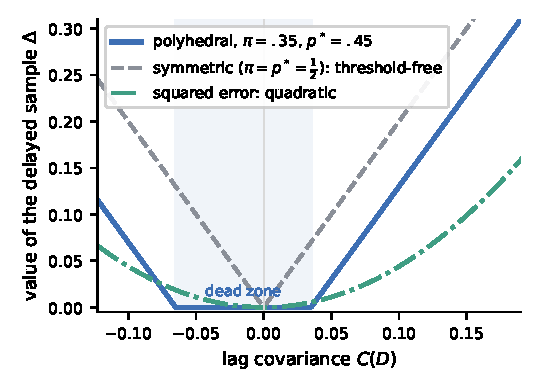
\includegraphics[width=.72\linewidth]{fig_trichotomy.pdf}
\caption{The contact-order trichotomy (Theorem~\ref{thm:contact}),
drawn exactly. Polyhedral objective with $\pi{=}.35$, one kink at
$p^*{=}.45$, $\Delta s{=}2$: sign-dependent hinges with dead-zone
thresholds $a^+{=}.035$ (positive branch) and $a^-{=}.065$ (negative
branch), so anticorrelation of the same magnitude can be worthless where
positive correlation has value. The symmetric case is the threshold-free
degenerate hinge; squared error responds quadratically with no dead
zone. The axis spans exactly the feasible covariance range
$[-\pi^2,\,\pi(1{-}\pi)]$; for stronger asymmetry (e.g.\
$\pi{=}.2$, $p^*{=}.3$) the negative-branch threshold exceeds the
feasible range entirely and anticorrelated sensing is worthless at
\emph{every} achievable covariance.}
\label{fig:trichotomy}\end{figure}
\subsection{Beyond polyhedral objectives: contact-order response}
\label{sec:smooth}

The polyhedral hypothesis is not decoration. For a continuous action set
$\psi$ is a supremum of \emph{infinitely} many affine functions and need
not be piecewise-linear, and the hinge law fails, constructively:

\begin{proposition}[Sq\kern0pt uared-error prediction: exactly q\kern0pt uadratic]
\label{prop:quadratic}
For $w\in[0,1]$ and $R(w,x)=-(w-x)^2$ (oscillation $\Omega=1$),
$\psi(p)=-p(1-p)$ is smooth and strictly convex, and, exactly,
\[
\Delta(D)\;=\;\operatorname{Var}(p_Y)\;=\;\frac{C(D)^2}{\pi(1-\pi)}:
\]
quadratic in the covariance, no hinge, no dead zone, for every $\pi$. More
generally, whenever $\psi$ is twice continuously differentiable near $\pi$
with $\psi''(\pi)>0$ (if the curvature vanishes the response is of higher
order; Theorem~\ref{thm:contact}),
\[
\Delta(D)\;=\;\tfrac12\,\psi''(\pi)\operatorname{Var}(p_Y)+o(C^2)
\;=\;\frac{\psi''(\pi)}{2\pi(1-\pi)}\,C(D)^2+o\bigl(C(D)^2\bigr).
\]
\end{proposition}
\begin{proof}
The optimal action under belief $p$ is $w=p$, so
$\psi(p)=-p(1-p)=p^2-p$; then
$\Delta=\E[\psi(p_Y)]-\psi(\pi)=\E[p_Y^2]-\pi^2=\operatorname{Var}(p_Y)$,
exact because $\psi$ is quadratic, and
$\operatorname{Var}(p_Y)=\pi(C/\pi)^2+(1-\pi)\bigl(C/(1-\pi)\bigr)^2
=C^2/\pi(1-\pi)$. The general statement is the second-order Taylor
expansion of $\psi$ at $\pi$ against the mean-$\pi$ posterior spread.
\end{proof}

Both regimes, and every intermediate one, are cases of a single
statement:

\begin{theorem}[Local response is set by the contact order]\label{thm:contact}
Suppose that near $\pi$,
\[
\psi(\pi+h)\;=\;\psi(\pi)+ah+c_+\,h_+^{\,q}+c_-\,(-h)_+^{\,q}+o(|h|^q)
\]
for some $q\ge1$ and $c_+,c_-\ge0$ not both zero. Then, as $C\downarrow0$,
\[
\Delta(C)\;=\;C^{\,q}\Bigl[c_+\,\pi^{1-q}+c_-\,(1-\pi)^{1-q}\Bigr]+o(C^{\,q}),
\]
and on the negative branch ($C\uparrow0$) the same with $|C|^q$ and the
weights $\pi\leftrightarrow(1-\pi)$ interchanged. If instead $\psi$ is
affine on a neighbourhood of $\pi$, then $\Delta(C)=0$ for all $|C|$ small
enough that both posteriors remain in that neighbourhood. This is the exact dead
zone.
\end{theorem}

\begin{proof}
The posteriors are $p_1=\pi+C/\pi$ (w.p.\ $\pi$) and $p_0=\pi-C/(1-\pi)$
(w.p.\ $1-\pi$); their mean is $\pi$, so the affine part of the expansion
cancels in $\Delta=\E[\psi(p_Y)]-\psi(\pi)$. For $C>0$ the $h_+^q$ term
contributes $\pi\,c_+(C/\pi)^q=c_+C^q\pi^{1-q}$ through $p_1$ and the
$(-h)_+^q$ term contributes $(1-\pi)\,c_-(C/(1-\pi))^q=c_-C^q(1-\pi)^{1-q}$
through $p_0$; both posterior deviations are $\Theta(C)$, so the $o(|h|^q)$
remainder is $o(C^q)$. For $C<0$ the posteriors trade sides of $\pi$,
exchanging the weights. The affine case is immediate.
\end{proof}

\begin{remark}[The trichotomy, as leading cases]\label{rem:trichotomy}
The three named regimes (dead zone, linear at a kink, quadratic under
smooth curvature) are precisely De~Lara and Gossner's small-information
trichotomy (\cite{delaragossner}, Thms.~3, 5 and 7, illustrated in their
Prop.~10), and their exact zero-value
characterization (their Prop.~2, the confidence-set condition) is the
posterior-space form of our dead zone. Theorem~\ref{thm:contact} adds
what their bounds deliberately do not: \emph{exact leading coefficients}
(their two-sided constants ``depend on the global behavior of the
value function, and hence cannot be inferred from local properties only,''
whereas in the delayed-binary geometry the coefficient
$C^q[c_+\pi^{1-q}+c_-(1-\pi)^{1-q}]$ is explicit), together with
general fractional contact orders $q\in(1,2)$, realizable by valid
suprema of affine rewards, and the lag-covariance parametrization with
its sign asymmetry. Each case fixes how weak
dependence buys value: \emph{prior on a kink}
$\Rightarrow$ linear response $\Delta\propto|C|$; \emph{prior interior to a
flat piece} $\Rightarrow$ dead zone, $\Delta=0$ until a threshold;
\emph{smooth curvature} $\Rightarrow$ quadratic response
$\Delta\propto C^2$. The companion's law is the first case. Symmetry
puts the prior on the decision kink, the polyhedral configuration
yielding threshold-free linear response. The dead zone is the sharp polyhedral form of the
Radner--Stiglitz nonconcavity of the value of information
\cite{radnerstiglitz84,chadeschlee02}, whose smooth setting is our third case (zero
marginal value at zero information, but not identically zero). And the
sign-dependence of Theorem~\ref{thm:hinge} means even the \emph{direction}
of correlation matters away from symmetry: with $\pi=0.2$ and one kink at
$p^*=0.3$, covariance $+0.03$ clears its threshold $(0.1)(0.2)=0.02$ and
has value, while $-0.03$ sits inside its threshold $(0.1)(0.8)=0.08$ and is
worthless.
\end{remark}

\begin{corollary}[The companion law, and why it is threshold-free]
For the symmetric chain ($\pi=\tfrac12$) with the $0/1$ prediction
objective ($K{=}1$, $p^*=\tfrac12$, $\Delta s=2$):
$a^{\pm}=0$ and $|C(D)|=\tfrac14 |r(D)|$, so
$\Delta(D)=2\cdot\tfrac14 |r(D)|=\tfrac12 |r(D)|$, the exact law of
\cite{infocom}. Symmetry places the prior \emph{on} the kink, the polyhedral
configuration with no dead zone; the linear-in-$r$ law is the degenerate
hinge.
\end{corollary}

\begin{remark}[The dead zone is a prediction, not a curiosity]
For $\pi\neq p^*$ the hinge says weakly-correlated delayed feedback is
\emph{worthless}, not slightly valuable, until $|C(D)|$ crosses
its branch threshold $a^{\pm}$: below threshold, both posteriors fall on one side of the decision
kink and the optimal action never changes. Operationally: a rare-event
admission controller ($\pi$ small, $p^*$ moderate) gains \emph{nothing}
from telemetry until the covariance clears the \emph{branch} threshold:
$C(D)>(p^*-\pi)\pi$ for positive correlation, but
$-C(D)>(p^*-\pi)(1-\pi)$ for negative. For rare events
($\pi$ small) the negative-branch threshold is larger by the factor
$(1-\pi)/\pi$, so anticorrelated telemetry must be far stronger before
it is worth anything. This is an exact, testable, sign-dependent cutoff for
when to stop paying for freshness at all. None of the envelopes of \S\ref{sec:comparison} see
this: the dead zone is a fact about geometry (posteriors vs.\ kink), which
is precisely what scalar information summaries discard
(Proposition~\ref{prop:noneq}).
\end{remark}

\begin{remark}[Beyond two states: a layer-cake decomposition, and the boundary]
For capacities $a_t\in\{0,\dots,C\}$ with monotone threshold objectives, the
objective decomposes over layer indicators $x^u_t=\mathbf 1[a_t\ge u]$, each
layer a binary experiment governed by its hinge (sketch in
Appendix~\ref{app:companion}). Against a comonotone static budget at matched
over-admission, a layer with $r_u\ge0$ contributes $\pi_u r_u(D)$, because
at matched surplus each layer's kink sits at its own prior and no layer has a
dead zone. This is a matched-surplus benchmark gain, not the Bayes envelope
of~\eqref{eq:envelope}. The companion leaves integer capacity open: the
per-layer decisions must stay nested to form one admission window, and
without a monotonicity condition the layerwise sum is only an upper bound
on the jointly feasible advantage. We do not close that gap here.
Effective one-dimensionality of the posterior family (a scalar belief
per layer, moved along a line by the observation) is a principal
tractable regime in which scalar closed forms arise; the
two-bit construction of Proposition~\ref{prop:noneq} is the minimal
experiment whose posterior geometry is irreducibly two-dimensional, and there
the value ceases to be a function of any scalar summary of dependence,
correlation or information alike.
\end{remark}

\section{Closed loop: what transfers, and what does not}\label{sec:closedloop}

The theory so far assumes the action does not move the state. In a
closed loop it does: an admission controller changes the queue it will
observe, and a sender changes the congestion it will be told about. Let the
state evolve as $X_{t+1}\sim P(\cdot\mid X_t,w_t)$, let the step-$t$ reward be
$R_t(w_t,X_t)$ with oscillation $\Omega$, and let a policy $\pi$ choose $w_t$ from
the controller's information $G_t$ (the delayed observations and its own
past actions). The action at step~$t$ is taken after $X_t$ is realized and
moves only later states.

\begin{proposition}[The per-step envelope survives closing the loop]\label{prop:clstep}
Fix any policy $\pi$ and a step $t$. Holding $\pi$ fixed at every other step, let
$\Delta^\pi_t$ be the gain in expected step-$t$ reward of the best
$G_t$-measurable action over the best constant action. Then
\[
0\;\le\;\Delta^\pi_t\;\le\;\Omega\sqrt{\tfrac12\,I^\pi(X_t;G_t)},
\]
where $I^\pi$ is the mutual information under the joint law that $\pi$
induces on $(X_t,G_t)$.
\end{proposition}

\begin{proof}
Changing only the step-$t$ action does not change the joint law of
$(X_t,G_t)$, which is fixed by the earlier steps. The step-$t$ reward is
$R_t(w_t,X_t)$, so the comparison is a one-step decision under that law,
and Theorem~\ref{thm:mi} applies to it.
\end{proof}

So every decision-value statement of \S\S\ref{sec:mi}--\ref{sec:multistate} holds in
closed loop, provided the information is measured under the law the
controller itself induces. What fails is the step from per-step decision
value to total value, because a closed-loop controller can use delayed
information to steer the state rather than to predict it.

\begin{proposition}[Steering has no information envelope]\label{prop:clsteer}
There is a controlled binary process with a reward of oscillation
$\Omega=1$ and delay $D=1$ such that, over $T\ge2$ steps, the best delayed-feedback
policy earns $(T-2)/2$ more than the best open-loop policy, while under that
feedback policy $\Delta^\pi_t=0$ at every step and the per-step envelopes
$\Omega\sqrt{\tfrac12 I^\pi(X_t;G_t)}$ sum to $\sqrt{(\ln 2)/2}\approx0.589$.
\end{proposition}

\begin{proof}
Let $X_0$ be a fair bit, $X_{t+1}=X_t\oplus w_t$ with $w_t\in\{0,1\}$, and
$R_t(w,x)=\mathbf 1[x=1]$, which does not depend on $w$, so
$\psi$ is linear at every step and $\Delta^\pi_t=0$ for every policy. An
open-loop policy leaves each $X_t=X_0\oplus c_t$ a fair bit and earns
$T/2$. With $G_t=(X_{t-1},w_0,\dots,w_{t-1})$ the controller knows
$X_t=X_{t-1}\oplus w_{t-1}$ from step~1 on; setting $w_1=1\oplus X_1$ and
$w_t=0$ afterwards holds $X_t=1$ for $t\ge2$ and earns $1+(T-2)=T-1$, which is
optimal because $X_0$ and $X_1$ are fair bits whatever is done before any
observation. Under this policy $G_0$ is trivial, $X_1$ is a fair bit
determined by $G_1$, and $X_t$ is constant for $t\ge2$, so the only
nonzero envelope is $\sqrt{(\ln 2)/2}$ at $t=1$.
\end{proof}

The pair draws the boundary precisely. Delayed information has a
decision value, which the envelope bounds in open and closed loop alike,
and a steering value, which it does not bound. The second is the subject
of control under communication constraints \cite{tatikondamitter04}, where
the information a controller needs is set by how fast the plant drifts
from its target, not by how much the past predicts the present. A
closed-loop instance of both is measured in \S\ref{sec:queue}.

\section{The law and its envelopes across domains}\label{sec:battery}

The companion paper had room for one paragraph of this study; the full
protocol and results are reported here. The question has two halves. First,
\emph{single-sample sufficiency}: on real binary state processes, does
history beyond the single delayed sample add decision value beyond the
\emph{exact empirical single-sample Bayes value}, computed from the
pooled $2{\times}2$ lag table with no symmetry assumption, so that
Theorem~\ref{thm:hinge}'s imbalance effects (dead zones included) are
carried automatically? Second, \emph{the envelope}: does the measured value
respect, and how tightly does it approach, the predictive-information bound
of Theorem~\ref{thm:mi}?

One caution frames everything that follows. Every battery quantity is a
property of the empirical mixture a series samples. A history gain pooled
over a whole record can come from identifying the regime as well as from
prediction within one (Lemma~\ref{lem:regime}), and every series here rejects
a homogeneous lag-1 law across calendar blocks, so the section reports the
pooled results and the block results side by side.

\subsection{Protocol}

Throughout this section, ``registered'' means fixed in the protocol code
before the final analysis runs (the introduction calls this protocol-fixed). The battery was not preregistered with a
third party, and its protocol was revised during the v3 and v4
development runs, whose record is part of the released artifact.

\textbf{Stationarity.} The envelopes of \S\ref{sec:mi} need no stationarity.
The covariance parametrization of \S\ref{sec:multistate}, the fitted homogeneous
Markov null, and the empirical dead-zone threshold all assume stationary
marginals, and the GOES and seismic series are plausibly piecewise
stationary at best. Pooling a long nonstationary series can make history
valuable because it identifies the regime or the time, not because of
stationary higher-order dependence. We therefore read every battery
quantity, including the seismic certificate, as a property of the
empirical mixture the series samples, not as a parameter of a stationary
process. Lemma~\ref{lem:regime} makes the distinction exact: a history gain
pooled over the whole record bounds what history reveals about the regime
plus what it predicts within one, and a gain measured inside a calendar
block bounds the second term alone; the regime analysis at the end of this
section measures both.

\textbf{Artifact.} An anonymized artifact is available for review at
\url{https://osf.io/273mh/overview?view_only=0b9598b1fdd84fd88688089e3408cfd1}
and will be archived on Zenodo on acceptance: the code, the derived binary
series, every result file, the Lean proof-check logs and MATLAB
symbolic-verification logs, the seeds of every resampling step, a
verification record for every reference, and a notebook that rebuilds
every table and figure from the result files and checks each printed
certificate (all 338 checks pass).

\textbf{Use of generative AI.} An AI assistant (Claude, Anthropic) was used
throughout as a research assistant, in the following specific ways. It
wrote, under the author's direction, the battery drivers (versions 3 to
5c), the stationarity and BGP analysis scripts, and the figure script, and
it ran them on the author's workstation. It drafted the protocol for the
BGP series and the stationarity check, which the author approved before any
data were fetched. It reviewed the proofs by independent re-derivation,
audited every reported number against the result files, and searched the
literature for prior statements of the results (the attribution of
Theorems~\ref{thm:mi} and~\ref{thm:incr} came from that search). It wrote
the Lean scripts that machine-check the finite and algebraic results and
the MATLAB scripts that symbolically verify the analytic results, and it drafted and copy-edited text. The author chose the
questions, the theory and the battery design, checked the outputs, and is
responsible for every claim.

\textbf{States.} Binary regime series from four physical domains, one
computer system, and controls: acoustic source azimuth and voice activity (LOCATA; azimuth at 120\,Hz, voice activity at 100\,Hz);
sperm-whale coda type (Dominica corpus, per-exchange); GOES space-weather
series (X-ray flux, magnetometer, proton flux; 1--5-minute cadence); seismic
ground motion at station IU.ANMO (1~Hz over 3.5 hours, from 30 minutes
before the origin of the 2015 Mw~8.3 Illapel, Chile earthquake, so the
record holds the teleseismic arrivals and their coda); BGP control-plane
activity at RIPE RIS collector rrc06 (1-minute, 1 to 7 September 2026,
state 1 when the minute's count of announced or withdrawn prefixes exceeds
the week's median, a rule registered before the data were fetched); a synthetic two-state Markov chain
(flip probability $0.02$) as positive reference; an i.i.d.\ fair-bit series
as null. Each series is binarized by the domain's registered thresholding
(the companion study's preparation scripts, unchanged).

\textbf{The two estimands.} For each lag $D$ on a per-domain grid:
(i) the \emph{exact empirical single-sample Bayes value}
$\widehat V_1(D)=\sum_y \hat w_y \max(\hat p_y, 1-\hat p_y)
-\max(\hat\pi,1-\hat\pi)$, the plug-in of \eqref{eq:envelope} for
$Y=X_{t-D}$ computed from the pooled lag table. For a balanced series
this is $\tfrac12|r(D)|$, and for an imbalanced one it carries
Theorem~\ref{thm:hinge}'s thresholds automatically (the per-domain class
proportion $\hat\pi$ is reported alongside); (ii) the value of the best
\emph{delayed-history} policy: a $k{=}6$-lag lookup predictor trained and
evaluated by blocked cross-validation (5 folds, contiguous blocks),
reported as accuracy above the \emph{best static (majority) policy}
$\max(\hat\pi,1-\hat\pi)$, the correct static benchmark; accuracy above
$\tfrac12$ overstates value whenever $\hat\pi\neq\tfrac12$. The
\emph{history gain} is the difference (ii)$-$(i).

\emph{Scope of the estimand.} Estimand (ii) is the value of one
\emph{registered policy class} $\mathcal P$ (six-lag lookup), i.e.\
$\widehat\Delta_{\mathcal P,W}=\sup_{\pi\in\mathcal P}V(\pi;W)
-V_{\mathrm{stat}}$, \emph{not} the Bayes history value $\Delta_W$ of
Theorem~\ref{thm:incr}. The asymmetry matters. Since
$V(\pi;W)\le V^\star_W$ for every $\pi$, any demonstrated improvement over
the exact single-sample value lower-bounds $\Delta_W-\Delta_Z$, so
\emph{positive} certificates transfer upward and the conditional-information
witnesses below are sound. \emph{Negative} findings bound only the class:
where the lookup policy finds nothing, some richer policy class could still
extract history value, so verdicts of that kind are stated as ``no
additional value detected by the registered six-lag lookup policy,'' never
as unrestricted single-sample sufficiency.

\textbf{Surrogate calibration.} The null for ``history adds nothing beyond
the law'' is a population of Markov surrogates per domain, each matched
to the real series' lag-1 transition probabilities and evaluated by the
identical pipeline, with $M=299$ surrogates. We name the procedure
precisely: because the surrogates are generated from \emph{estimated}
lag-1 transition probabilities, this is a \emph{parametric-bootstrap test
under a fitted Markov null} (not an exact randomization test for the
broad null ``history adds nothing''), with
$p=(1+\#\{T_j\ge T_{\mathrm{obs}}\})/(M+1)$ (smallest reportable value
$1/300\approx0.0033$, written $p<.004$, never $.00$), together with the
companion study's practical floor of $0.03$ on the effect. Because each
surrogate is Markov, its true history gain is zero and its own exact
$\widehat V_1$ is computable from its lag table, so the $M$ surrogate gain
estimates sample the pipeline's estimation error $E$ \emph{under the
fitted Markov model}. The two tails play different roles: a lower
certificate needs the \emph{over}-estimation tail,
$\varepsilon_{\mathrm{over}}=q_{0.95}(E)$, giving
$L=\hat g-\varepsilon_{\mathrm{over}}$; an upper (equivalence) bound needs
the \emph{under}-estimation tail,
$\varepsilon_{\mathrm{under}}=-q_{0.05}(E)$, giving
$U_2=\hat g+\varepsilon_{\mathrm{under}}$; the two coincide only under a
symmetry condition, so both are computed and reported separately. Both
are \emph{model-calibrated} (not distribution-free) bounds. Complementing
them, the analysis reports a \emph{dependence-aware} moving-block
bootstrap on held-out paired loss differences, comparing the registered $k{=}6$
policy against the pooled-\emph{exact} single-sample policy (in-sample
fit favouring the single-sample arm, hence conservative for the
incremental value), blocks resampled within runs at the selected lag
$D^*$. Because $D^*$ is an argmax over the lag grid that the bootstrap
treats as fixed, the i.i.d.\ null's paired interval calibrates the
\emph{selection} bias not covered (its upper end $\approx0.02$); paired
lower bounds are claimed only above that floor. The selection-aware
refinement has been executed: repeating the entire lag selection inside
each block-bootstrap replicate (blocks resampled with shared starts
across all registered lags, the maximizing lag re-selected per replicate,
the one-sided bound taken from the resulting max-statistic distribution).
The i.i.d.\ null quantifies the percentile-of-max procedure's residual
optimism at $+0.008$, so certificates are claimed only where the
parametric-bootstrap detection test also fires, which excludes the
noisy short-series maxima the winner's curse can manufacture (whale,
protons). Validity checks pass:
the Markov reference's interval straddles zero (no phantom conditional
information) and azimuth's is slightly negative (the overfitting cost of
the richer class).
In plain terms: choosing the best of many lags and then quoting its
interval overstates the gain, because the best lag is partly the luckiest.
The fixed-lag bound $L^{\mathrm{blk}}_{D^*}$ ignores that choice; the
selection-aware bound $L^{\mathrm{blk}}_{\max}$ repeats the choice inside every
bootstrap replicate, so it bounds the gain of whichever lag wins, and the
i.i.d.\ null, which has no true gain at any lag, shows how much optimism
remains ($+0.008$).

\textbf{The practical floor.} Every verdict compares a bound with a
practical floor of $0.03$. On the $0/1$ prediction objective ($\Omega=1$)
the gain is a difference in the probability of a correct decision, so the
floor is three percentage points of correct decisions per decision. It was
fixed with the equivalence rule before the final runs, and it sits above
the procedure's own false-positive floor, the upper end of the i.i.d.\ null's
paired interval ($\approx0.02$), and above the selection-aware residual
optimism ($+0.008$). It does not come from a cost model, so
we report how the verdicts move with it. Seismic is ``history adds'' at
floors of $0.02$, $0.03$ and $0.05$. BGP is ``history adds'' at $0.02$ and
$0.03$ and only detected at $0.05$, where its lower bounds ($+.044$,
$+.047$) fall short. Magnetometer becomes ``history adds'' at $0.02$; at
$0.05$ the whale codas and protons become equivalent (Table~\ref{tab:floor}).

\begin{table}[h]\centering\footnotesize
\begin{tabular}{lccc}
\toprule
Series & floor $0.02$ & floor $0.03$ (used) & floor $0.05$ \\
\midrule
LOCATA azimuth & not established & equivalent & equivalent \\
Sperm-whale codas & inconclusive & inconclusive & equivalent \\
GOES protons & not established & not established & equivalent \\
GOES X-ray flux & detected (exploratory) & detected, below floor & detected, below floor \\
GOES magnetometer & history adds & detected (exploratory) & detected, below floor \\
Seismic ANMO & history adds & history adds & history adds \\
BGP rrc06 & history adds & history adds & detected (exploratory) \\
\bottomrule
\end{tabular}
\caption{Verdicts at three practical floors, from the same result files.
Series not listed (two-state Markov, LOCATA VAD) are equivalent at every
floor, and the i.i.d.\ null is the selection control throughout.}
\label{tab:floor}
\end{table}

\emph{Non-rejection is not exactness}: where the test does not fire, we
report the model-calibrated two-tail upper bound
$U_2=\text{gain}_{\max}+\varepsilon_{\mathrm{under}}$ and claim ``no
detectable excess (equivalent within the margin)'' only when $U_2<0.03$.

\textbf{The two information measurements.} For each domain and lag, the
plug-in $\widehat I(X_t;X_{t-D})$ from pooled pair counts ($2{\times}2$;
first-order plug-in bias $O(1/N)$, negligible at the pooled sample sizes
reported) and the envelope $\sqrt{\widehat I/2}$. Their registered uses
follow the two theorems, matched to the observable each governs.
\emph{Single sample} (Theorem~\ref{thm:mi} at $Y=X_{t-D}$): the exact
$\widehat V_1$ must respect $\sqrt{\widehat I/2}$, a population identity
whose empirical check is a consistency diagnostic. \emph{History}
(Theorem~\ref{thm:incr}): the history policy observes the \emph{window},
so the single-lag envelope does not bound it. A history value above
$\sqrt{\widehat I_1/2}$ is not a violation but exactly what genuine
higher-order dependence should produce. The history gain over
$\widehat V_1$ is a registered-policy gain that \emph{lower-bounds} the
Bayes increment $\Delta_W-\Delta_Z$, and its model-calibrated lower
bound therefore also bounds \emph{conditional} predictive information:
\[
I(X_t;\,\text{history}\mid X_{t-D})\;\ge\;
2\,\bigl[(\text{gain}_{\max}-\varepsilon_{\mathrm{over}})^{+}\bigr]^{2},
\]
never through the raw point estimate, whose positive noise would inflate
the certificate. The total-information witness
$I(X_t;\text{window})\ge2[(\widehat\Delta_{\mathrm{hist}}
-\varepsilon_{\mathrm{over}})^{+}]^{2}$ is retained separately, with the
caveat that its estimator differs from the incremental-gain estimator and
in principle requires its own overestimation calibration; the gain-error
quantile is reused as an approximation and labelled as such.

\subsection{Results}

Table~\ref{tab:battery} reports the final analysis
from four analysis runs of the released artifact. Run v5 gives the gains,
$p$ and calibration tails, v5b the fixed-$D^*$ bounds and v5c the
selection-aware bounds. Run v4 gives the single-sample quantities
$\widehat V_1$ and $\widehat I$, the tightness ratios,
Fig.~\ref{fig:tightness} and the total-information witness. The BGP series and the calendar-block
analysis come from separate runs of the same code, registered in the
artifact before the BGP data were fetched. The v3 run and the
protocol corrections are preserved in the artifact. Per domain: the class proportion $\hat\pi$; the
maximum history-class gain over the exact single-sample Bayes value
$\widehat V_1$; the parametric-bootstrap $p$ under the fitted Markov null
($M{=}299$, floor $1/300$, written $<.004$); the two calibration tails
$\varepsilon_{\mathrm{over}}=q_{0.95}(E)$ and
$\varepsilon_{\mathrm{under}}=-q_{0.05}(E)$; the two-tail equivalence
bound $U_2=\text{gain}_{\max}+\varepsilon_{\mathrm{under}}$
(margin $0.03$); and the dependence-aware paired interval, a
moving-block bootstrap (blocks within runs, $B{=}2000$) of the per-position
loss difference between the registered $k{=}6$ policy and the
pooled-\emph{exact} single-sample policy at the selected lag $D^*$, the
exact-arm fit favouring the single-sample side so the interval is
conservative for the incremental value.

\begin{table}[h]\centering\footnotesize
\begin{tabular}{lrrrrrrcl}
\toprule
Domain & $\hat\pi$ & gain & $p$ & $\varepsilon_{\mathrm{ov}}$ &
$\varepsilon_{\mathrm{un}}$ & $U_2$ & $L^{\mathrm{blk}}_{D^*}\,/\,L^{\mathrm{blk}}_{\max}$ & verdict \\
\midrule
Two-state Markov & $.470$ & $+.000$ & $.78$ & $.006$ & $.000$ & $.000$ & $-.003\,/\,+.000$ & equivalent \\
i.i.d.\ null & $.497$ & $+.012$ & $.023$ & $.011$ & $-.001$ & $.011$ & $+.005\,/\,+.008$ & selection control \\
LOCATA azimuth & $.494$ & $+.008$ & $.063$ & $.009$ & $.020$ & $.027$ & $-.003\,/\,-.001$ & equivalent \\
LOCATA VAD & $.636$ & $-.000$ & $.82$ & $.052$ & $.000$ & $.000$ & $.000\,/\,.000$ & equivalent \\
Sperm-whale codas & $.483$ & $+.046$ & $.997$ & $.117$ & $-.063$ & $-.016$ & $+.010\,/\,+.040$ & inconclusive$^{\ddagger}$ \\
GOES protons & $.489$ & $+.029$ & $.11$ & $.033$ & $.003$ & $.032$ & $+.002\,/\,+.020$ & not established \\
GOES X-ray flux & $.421$ & $+.028$ & $<.004$ & $.008$ & $.001$ & $.028$ & $+.011\,/\,+.017$ & detected, below floor \\
GOES magnetometer & $.456$ & $+.033$ & $<.004$ & $.010$ & $.001$ & $.033$ & $+.022\,/\,+.026$ & detected (exploratory) \\
Seismic ANMO & $.508$ & $+.158$ & $<.004$ & $.014$ & $.000$ & $.158$ & $\mathbf{+.146\,/\,+.145}$ & history adds \\
BGP rrc06 & $.500$ & $+.053$ & $<.004$ & $.015$ & $-.002$ & $.051$ & $+.044\,/\,+.047$ & history adds \\
\bottomrule
\end{tabular}
\caption{Battery v5 (final analysis). Verdicts are statements about the
\emph{registered six-lag lookup class}. ``Detected'' means the
parametric-bootstrap $p$ is at its floor ($<.004$); no series has $p$
between $.004$ and $.023$, so any level in that range gives the same
verdicts. This is a conservative analysis rule adopted during the final
analysis, not a preregistered significance level. The verdicts, applied
in this order: ``history adds'' $=$ detected, with both moving-block lower
bounds above the practical floor $0.03$ (a certificate is issued);
``detected (exploratory)'' $=$ detected, point gain above the floor, lower
bounds below it; ``detected, below floor'' $=$ detected, point gain at or
below the floor; ``equivalent'' $=$ not detected and $U_2<0.03$;
``not established'' $=$ not detected and $U_2\ge0.03$; ``inconclusive''
$=$ the calibrations disagree (footnote). Detection takes precedence, so
X-ray, which also has $U_2<0.03$, is reported as detected. ``Exploratory''
refers to the size of the gain, not to the calendar-block analysis. The i.i.d.\ null ($p=.023$) is the selection control. $L^{\mathrm{blk}}_{D^*}$ and $L^{\mathrm{blk}}_{\max}$ are the
one-sided 95\% moving-block lower bounds at the pre-selected lag and
with lag selection repeated inside each replicate (the latter bounds the
\emph{maximal} gain over the grid).
$^{\ddagger}$Inconclusive: the calibrations disagree. The fitted-Markov
calibration finds the estimator biased upward ($U_2<0$), while both
moving-block lower bounds are positive and the selection-aware one
($+.040$) exceeds the practical floor, and the detection test does not
fire on this short series ($p=.997$; $N=4{,}698$ pairs, the second-shortest,
Table~\ref{tab:details}). We claim neither equivalence nor a certificate. The i.i.d.\ null's \emph{positive} paired interval is the
empirical lag-selection bias (its upper end, $\approx0.02$, is the claim floor for
paired bounds, since $D^*$ is an argmax the bootstrap treats as fixed).
Bold: the one interval that dwarfs every calibration concern. Sample sizes, lag grids, selected lags and block lengths are in Table~\ref{tab:details}.}
\label{tab:battery}
\end{table}

\begin{figure}[t]\centering
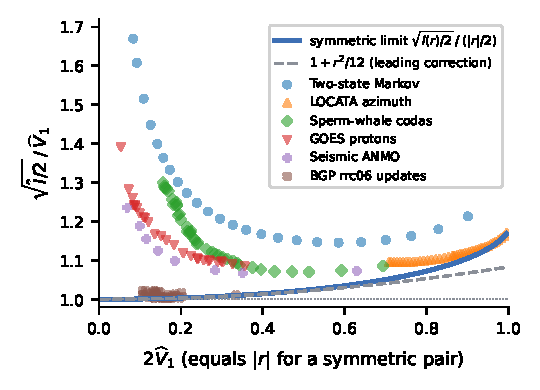
\includegraphics[width=.72\linewidth]{fig_tightness.pdf}
\caption{Tightness of the information envelope on approximately
balanced binary pairs (Proposition~\ref{prop:tight}). Points: per-lag ratio
$\sqrt{\hat I/2}\,/\,\widehat V_1$ of the information envelope to the exact
single-sample value, both computed from the same pooled lag table, for
the series with $|\hat\pi-\tfrac12|<.035$ (lags with $\widehat V_1>.025$; the
i.i.d.\ null has none). Theorem~\ref{thm:mi} applied to that table forces every
point to at least one. The horizontal axis is $2\widehat V_1$, which equals
$|r|$ for a symmetric pair, so the curve is the symmetric limit
$\sqrt{I(r)/2}\,/\,(|r|/2)$ and the dashes its leading correction
$1+r^2/12$. Points above the curve at small $\widehat V_1$ are the mildly
imbalanced series, whose single-sample value is pulled toward
Theorem~\ref{thm:hinge}'s threshold (Fig.~\ref{fig:trichotomy}). A consistency
check, not an independent test.}
\label{fig:tightness}\end{figure}

Four readings, in increasing order of consequence.

\begin{figure}[t]\centering
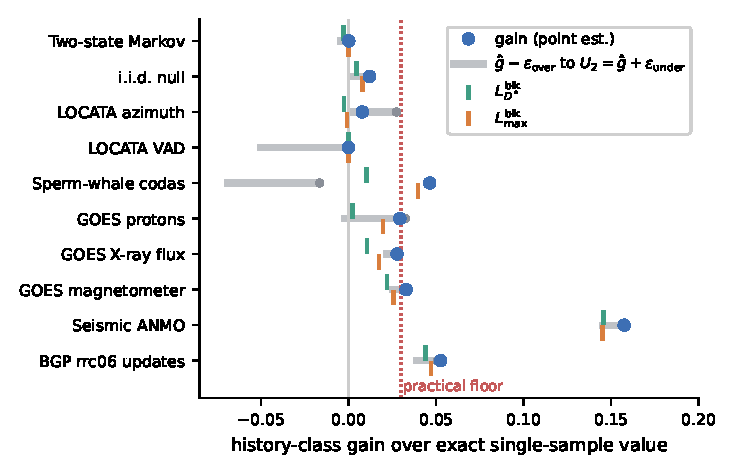
\includegraphics[width=.9\linewidth]{fig_battery.pdf}
\caption{The battery at a glance. Dots: maximum history-class gain over
the exact single-sample value; grey bars: the model-calibrated interval
$[\hat g-\varepsilon_{\mathrm{over}},\hat g+\varepsilon_{\mathrm{under}}]$;
ticks: the one-sided 95\% moving-block bounds ($B=2000$ replicates) at
fixed $D^*$ (upper, teal) and with in-replicate lag selection (lower,
orange); solid vertical line: zero; dotted vertical line: the registered
practical floor $0.03$. Seismic and BGP separate from both
zero and the floor; the i.i.d.\ null's positive selection-aware tick
is the empirical winner's-curse floor; whale's wide bar is the
short-series noise the verdict language respects. Where
$\varepsilon_{\mathrm{under}}<0$ (whale, i.i.d.) the bias-corrected
upper endpoint $U_2$ sits \emph{below} the point estimate, because the
estimator is upward-biased there, and the bound says so.}
\label{fig:battery}\end{figure}

\textbf{The protocol corrections changed the conclusions.}
Under the original chance baseline, four series appeared to carry history
value beyond the single sample (gains $0.100$--$0.367$). Under the
majority baseline and exact $\widehat V_1$: VAD's gain vanished entirely
($+0.100\to-0.000$; $\hat\pi=.636$, so the whole effect was the
majority-class head start), X-ray shrank $0.185\to0.028$, magnetometer
$0.147\to0.033$, and only seismic survived at strength
($0.367\to0.158$). The two-tail calibration then \emph{strengthened}
the equivalence side: $\varepsilon_{\mathrm{under}}$ is near zero or
negative on most series, so VAD joins the class-equivalent block. On the
whale codas the two calibrations point in opposite directions, and that
series is reported as inconclusive. Sub-unity ratios of the envelope to the exact
single-sample value disappeared with the imbalance correction. On the
series with $|\hat\pi-\tfrac12|<.035$ the median ratio
$\sqrt{\hat I/2}/\widehat V_1$ runs from $1.01$ (BGP) to $1.35$ on the six
such series, above one as
Theorem~\ref{thm:mi} requires. This is a consistency check, not an
independent test, since $\hat I$ and $\widehat V_1$ come from the same
pooled lag table. In Fig.~\ref{fig:tightness}, the points above the symmetric
limit at small $\widehat V_1$ are the mildly imbalanced series.

\textbf{The controls behave as designed.} The i.i.d.\ null has no true
history value, and its positive bounds ($+.005$ fixed-lag, $+.008$
selection-aware) are the procedure's false-positive floor, which every
claimed gain must clear. The two-state Markov reference, whose single
delayed sample is sufficient by construction, comes out equivalent. VAD's
fixed-lag entry is exactly zero for a structural reason: at its selected
lag of one step the six-lag lookup policy and the exact single-sample
policy reduce to the same majority rule on every fold.

\textbf{Two series exhibit material history gains.} Seismic and BGP are
detected with both moving-block lower bounds above the practical floor. X-ray
and magnetometer show smaller statistically detected gains near the
registered practical threshold (point gains $.028$ and $.033$ against
$.03$, lower bounds below it); on the remaining series \emph{no
additional value was detected by the registered six-lag lookup policy},
with class equivalence established where $U_2<0.03$ and withheld
where it is not (protons, $U_2=.032$). None of these negative findings
asserts unrestricted single-sample sufficiency: a richer policy class
could in principle extract value the lookup class does not
(\S~protocol, scope of the estimand).

\textbf{An empirical dead zone.} The imbalanced GOES series exhibit
Theorem~\ref{thm:hinge}'s geometry at the plug-in level: X-ray
($\hat\pi=.421$, kink at $\tfrac12$, positive-branch threshold
$a^+\approx0.033$) has $\widehat V_1$ exactly zero across its
moderate-covariance lags (the majority policy is unbeatable by any
single delayed sample), while its plug-in information remains positive:
\emph{information without value}, the phenomenon of
Proposition~\ref{prop:noneq}, on a physical series. (Population
uncertainty for the dead-zone boundary itself is future work; we label
this an \emph{empirical} dead zone.)

\textbf{The pooled conditional lower bounds.} By
Theorem~\ref{thm:incr}, each detected history gain converts into a lower
bound on conditional predictive information over its whole record. The \emph{primary} result is dependence-aware and
empirically selection-calibrated (the i.i.d.\ null measures the
procedure's residual optimism; we give no formal coverage argument for the
maximum), with the correctly-stated target: inference on the per-replicate maximum bounds the
\emph{maximal} gain over the registered lag grid, so the certificate
reads
$\max_{D\in\mathcal D} I(X_t;\text{history}_D\mid X_{t-D})
\ge 2(0.1453)^2\approx0.042$ nats ($0.061$ bits, about $6\%$ of the
entropy of a fair binary state, so a predictor that also reads the history
can lower its expected log-loss by at least that much). In words, \emph{there exists a registered
lag at which the conditional predictive information is at least
$0.042$ nats}. (A claim at the specific $D^*$ would need a simultaneous
band or sample splitting; the fixed-$D^*$ interval below is the
conditional-on-$D^*$ statement.) Two further routes
corroborate to within a few percent: the fixed-$D^*$ moving-block
interval ($[+.146,+.168]$, $\approx0.042$) and the fitted-Markov
surrogate calibration ($2(0.1575-0.0139)^2\approx0.041$), alongside the \emph{approximate} total-information witness
$I(X_t;\text{window})\gtrsim0.176$ nats ($0.254$ bits) (exploratory: its estimator
reuses the gain-error calibration, as noted in the protocol). The same
route gives BGP $2(0.0472)^2\approx0.0045$ nats (fixed-$D^*$ bound $+.044$;
surrogate route $2(0.0527-0.0154)^2\approx0.0028$). Magnetometer's selection-aware bound ($+.026$, certificate
$\approx0.001$ nats) is small and reported as exploratory. The instrument reads in
both directions: class equivalence or bounded excess on most series; a
dependence-aware conditional-information lower bound exactly where the
history structure is found.

\textbf{Regimes.} The stationarity check was registered with the BGP
series before its data were fetched: each of the five series with a
detection splits into three equal contiguous calendar blocks, and the
seismic certificate counts as block-robust only if its selection-aware
bound clears the practical floor in all three. \emph{It does not.} Block~1,
which is mostly the 30 minutes before the earthquake's waves arrive, gives
$+.014$ ($p=.45$, no detection), while blocks~2 and~3 give $+.219$ and
$+.165$, certificates of $0.096$ and $0.054$ nats, both larger than the
pooled $0.042$ (Table~\ref{tab:regimes}). BGP shows the same shape: a
detection below the floor in block~1, history adds in block~2 (certificate
$0.0062$ nats), and no material gain was detected by the registered lookup policy in block~3, while its class proportion drifts
from $.65$ to $.32$ under the single weekly threshold. The GOES detections
do not reach the bootstrap floor in any block, and a chi-square test
rejects equal lag-1 transition matrices across blocks for every series
($p\le10^{-4}$). By Lemma~\ref{lem:regime}, the pooled certificates bound
regime identification plus within-regime prediction, and the block
certificates isolate the second. On both the earthquake record and the
BGP week, the registered lookup policy detects material within-block value
in selected blocks and no material value in the remaining blocks; a richer
policy class could find value the lookup class does not. For a controller
this is the operational reading. The value of
delayed history is a property of the regime, and the instrument says
where it pays. The registered robustness test failed and is reported as
failed; the block results are descriptive.

\begin{table}[h]\centering\footnotesize
\setlength{\tabcolsep}{3pt}
\begin{tabular}{llrrrrl}
\toprule
Series & block & $\hat\pi$ & gain & $p$ & $L^{\mathrm{blk}}_{\max}$ & verdict \\
\midrule
Seismic ANMO & 1 & $.513$ & $+.012$ & $.45$ & $+.014$ & equivalent \\
 & 2 & $.501$ & $+.237$ & $<.004$ & $\mathbf{+.219}$ & adds (0.096 nats) \\
 & 3 & $.514$ & $+.181$ & $<.004$ & $\mathbf{+.165}$ & adds (0.054 nats) \\
BGP rrc06 & 1 & $.649$ & $+.010$ & $<.004$ & $+.001$ & below floor \\
 & 2 & $.527$ & $+.062$ & $<.004$ & $+.056$ & adds (0.006 nats) \\
 & 3 & $.323$ & $+.003$ & $.20$ & $-.003$ & equivalent \\
GOES X-ray & 1/2/3 & $.37$/$.42$/$.47$ & $+.020$/$+.036$/$+.006$ & $.017$/$.007$/$.66$ & $+.013$/$+.017$/$+.005$ & none detected \\
GOES magn. & 1/2/3 & $.47$/$.45$/$.45$ & $+.030$/$+.024$/$+.022$ & $.040$/$.057$/$.043$ & $+.019$/$+.028$/$+.001$ & none detected \\
GOES protons & 1/2/3 & $.50$/$.48$/$.48$ & $+.017$/$+.055$/$+.040$ & $.76$/$.12$/$.33$ & $+.003$/$+.026$/$+.027$ & none detected \\
\bottomrule
\end{tabular}
\caption{Registered calendar-block analysis (three equal contiguous blocks
per series; same pipeline and verdict rules as Table~\ref{tab:battery}). The
pre-stated seismic test (selection-aware bound above $0.03$ in every block)
fails in block~1. ``Adds'' means history adds, with its certificate. Both history-adds series carry their value in one or two
regimes, and the block certificates exceed the pooled ones where history
pays. Homogeneity of the lag-1 transition matrices is rejected for every
series (chi-square, df $=4$, $p\le10^{-4}$).}
\label{tab:regimes}
\end{table}

\subsection{A closed-loop queue}\label{sec:queue}

Section~\ref{sec:closedloop} separates decision value from steering value. To see
both on a system, we registered (before running it) a discrete-time
bottleneck queue with capacity $K=20$ in which the controller's own
packets change the occupancy it later observes. Each slot the sender
chooses to send or not and earns $w\,(1-2X_t/K)$, so sending pays while the
queue is short and costs while it is long; then its packet and
cross-traffic (probability $0.3$) arrive and one packet departs with
probability $0.5$. The controller sees the occupancy with delay $D$ and
knows its own past actions. We compare the best open-loop policy (send
with a fixed probability) with two delayed-feedback threshold policies,
one on the delayed occupancy alone and one on the delayed occupancy plus
the packets it has sent since; parameters are selected on two seeds and
every value below is measured on two held-out seeds of $2\times10^5$ slots
each. Under the selected feedback policy we compute, from the empirical
joint law it induces, the per-step decision value $\Delta$ of the statistic
(delayed occupancy, own recent sends) and its envelope
$\Omega\sqrt{\hat I/2}$ (Table~\ref{tab:queue}).

Three readings were fixed in advance. First, Proposition~\ref{prop:clstep}
predicts $\Delta\le\Omega\sqrt{\hat I/2}$ at every delay; it holds at all
eight, by three to four orders of magnitude. Second, the feedback gain
falls with every step in $D$, from $0.117$ to $0.013$ per slot, but has not
reached zero at $D=64$ (interval $[0.011,0.014]$): the count of the
controller's own recent sends is fresh even when the occupancy reading is
stale, and the policy that ignores it falls below open loop from $D=16$
on. Third, as a description, almost the whole gain is steering: the
steering share $1-\Delta/g_{\mathrm{dyn}}$ is at least $0.994$ at every delay.
The selected policies hold the queue at zero to two packets, where the
one-step choice is always to send, so the decision value nearly
vanishes: the controller has steered itself into a dead zone of its own
immediate decision. In this queue the per-step envelope happens to exceed
the dynamic gain at every delay; by Proposition~\ref{prop:clsteer} it need not,
and it bounds the decision part only.

\begin{table}[h]\centering\footnotesize
\begin{tabular}{rrrrrr}
\toprule
$D$ & $g_{\mathrm{dyn}}$ & $\hat I$ (nats) & $\Omega\sqrt{\hat I/2}$ & $\Delta$ & steering share \\
\midrule
0 & $0.117$ & $1.563$ & $1.768$ & $0.00004$ & $1.000$ \\
1 & $0.101$ & $0.747$ & $1.222$ & $0.00008$ & $0.999$ \\
2 & $0.087$ & $0.480$ & $0.980$ & $0.00007$ & $0.999$ \\
4 & $0.077$ & $0.304$ & $0.779$ & $0.00013$ & $0.998$ \\
8 & $0.062$ & $0.171$ & $0.585$ & $0.00017$ & $0.997$ \\
16 & $0.046$ & $0.091$ & $0.427$ & $0.00024$ & $0.995$ \\
32 & $0.028$ & $0.045$ & $0.302$ & $0.00014$ & $0.995$ \\
64 & $0.013$ & $0.030$ & $0.246$ & $0.00007$ & $0.994$ \\
\bottomrule
\end{tabular}
\caption{Closed-loop queue (registered; held-out seeds; values per slot).
$g_{\mathrm{dyn}}$: best delayed-feedback policy minus best open-loop policy
(open loop earns $0.083$); 95\% block-bootstrap intervals have half-width
at most $0.0014$. $\Delta$: per-step decision value of the controller's
statistic under the law its policy induces; $\Omega\sqrt{\hat I/2}$: the
envelope of Proposition~\ref{prop:clstep} with plug-in information. The
decision value stays under the envelope at every delay, and the gain is
almost entirely steering.}
\label{tab:queue}
\end{table}

\section{Related work}\label{sec:related}

\emph{Value of information.} The Bayes envelope is the classical object of
statistical decision theory \cite{howard1966,raiffa61}, and its convex
geometry is charted territory: De Lara and Gossner \cite{delaragossner}
study the value function as a support function, characterize
\emph{exactly} when information has zero value (their Prop.~2), and prove
the small-information trichotomy our Theorem~\ref{thm:contact}
generalizes (their Thms.~3, 5 and 7; see Remark~\ref{rem:trichotomy} for the
precise delta). Our Lipschitz lemma instantiates their payoffs--beliefs
duality; the sum-over-kinks skeleton of Theorem~\ref{thm:hinge} descends
from the mixture-of-primitives representations of statistical information
for binary experiments \cite{schervish89,reidwilliamson11}, and what is
new there is the exact lag-covariance parametrization with explicit
sign-asymmetric thresholds, a form we have not found in that
literature, nor in the nonconcavity strand
\cite{radnerstiglitz84,chadeschlee02,delaragilotte07,whitmeyer25}; the comparison-of-experiments order behind
Lemma~\ref{lem:blackwell} is Blackwell's \cite{blackwell53}; and the
Radner--Stiglitz nonconcavity \cite{radnerstiglitz84,chadeschlee02}
anticipates the zero-marginal-value onset in smooth settings; the exact
dead zone is its polyhedral counterpart. \emph{Minimum excess risk.} The envelope inequalities of
\S\ref{sec:mi} are published results of the minimum-excess-risk
literature: the unconditional bound in \cite{makhdoumi14,gyorfi23,xu20},
the conditional form in \cite{hafezkolahi21,xuraginsky22}, the proof
engine in \cite{russo16}; Fano-type families bounding Bayes \emph{error}
by information are the classical ancestors. That literature also
contains the exact logarithmic anchor (MER under log loss \emph{equals}
conditional information; \cite{xuraginsky22}, Lem.~2), which joins the
Kelly--Barron--Cover bracket below. What we have not found there, in the
economics of information or elsewhere, is the value-of-delayed-observation
framing, the exact covariance-parametrized laws of \S\ref{sec:multistate},
the envelope \emph{anchored to an exact law} (sharp to $O(r^3)$), its ordering against mixing
envelopes with both separations constructed, and its inversion into
certified conditional-information witnesses.

\emph{The logarithmic exception.} For log-utility gambling the value of
side information \emph{equals} mutual information: Kelly \cite{kelly56}
for the growth rate, Barron and Cover \cite{barroncover88} for the general
bound $\Delta\le I$ with equality characterizations. Log utility is
unbounded, escaping our $\Omega$-bounded class; the pair of results
brackets the landscape. Unbounded log utility buys equality, bounded
utility only an envelope, and Proposition~\ref{prop:noneq} shows the gap is
essential, not technical.

\emph{Age of information, and its critics.} AoI \cite{yates21} treats
freshness as the object, with sampling-policy results such as \cite{sun17}
optimizing age processes. That age alone lacks decision significance has
already been argued \emph{within} the field: age-of-incorrect-information
replaces the clock with an error-aware penalty \cite{maatouk20}, explicit
AoI-vs-VoI scheduling comparisons exist for networked control
\cite{ayan19}, and value-of-information metrics for feedback control have
been quantified directly, including an explicit derivation of the
value--age relation \cite{soleymani22,valueage24}. Our claim is accordingly not
that age lacks decision semantics (that point is established) but
more specific: for exogenous one-step bounded-reward decisions the exact semantic
object is the posterior Bayes envelope, which admits a universal
mutual-information converse, an explicit binary geometry (hinges, dead
zones, quadratic regimes), and an operational inversion into
predictive-information witnesses.

\emph{Delayed information in control.} Delayed-sharing information
structures go back to Witsenhausen \cite{witsenhausen68} and are
systematized by the common-information approach \cite{nayyar13}; remote
estimation studies the estimation face of the same trade
\cite{sun17}. Our setting is the tractable exogenous corner of that world
(the action does not affect the state), which is exactly what makes
closed forms and universal envelopes available.

\emph{Predictive information.} Bialek, Nemenman and Tishby
\cite{bialek01} study $I(\text{past};\text{future})$ as a measure of
process complexity. Theorems~\ref{thm:mi} and \ref{thm:hinge} are, in that
vocabulary, statements about what predictive information can and cannot buy
a bounded-utility decision maker, with the battery's witness bound
$I\ge 2[(\widehat\Delta-\varepsilon)^{+}]^2$ giving a one-sided lower bound on
predictive information from policy value alone.

\section{Conclusion}\label{sec:conclusion}

The companion paper measured one exact law on one system. This paper
locates that law inside a unified theory of exogenous one-step
bounded-reward decisions under delay: value of delayed
information is the Bayes envelope; the envelope is bounded by predictive
information (universally), by mixing (given a model), and by the entropy
of the observation (given nothing); for binary state it is a sign-dependent sum of hinges under polyhedral
objectives (a smooth value function giving quadratic weak-correlation
response instead), and exactly nothing (inside the dead
zone) when the prior sits off a kink and the coupling is weak. Beyond one effective dimension, no scalar summary of dependence
determines value at all. Each claim is falsifiable, and the ten-series
battery exercises the operational claims: the protocol-fixed policy shows
no detectable history excess where the model-calibrated equivalence
criterion is met; the information envelope holds on every real pair table
as a consistency check; policy gains yield dependence-aware lower bounds on
conditional predictive information; and calendar blocks identify where
those gains occur. The instrument reads in both directions; that, more
than any single inequality, is what we hope survives.

\appendix
\section{Companion results restated}\label{app:companion}

No claim in this paper depends on the companion. Every result used from it
is stated and proved below: the Lipschitz lemma (Lemma~\ref{lem:lip}), the
binary chain's mixing coefficient and exact law, and the layer-cake sketch.
Theorems~\ref{thm:mi}, \ref{thm:incr} and \ref{thm:hinge} are this paper's own
statements; the first two restate published inequalities (\S\ref{sec:mi})
and are proved in full in the text.

\paragraph{Mixing coefficient.} Throughout,
$\beta(D)=\E[\sup_{B\in\mathcal F_{\ge t}}
|\mathbb P(B\mid\mathcal F_{\le t-D})-\mathbb P(B)|]$ (event-supremum
convention; a lower bound for the absolute-regularity coefficient, so the
vacuousness results transfer conservatively).

\paragraph{Lipschitz value (Lemma~\ref{lem:lip}).} Let $\Omega\ge\sup_x R(w,x)-\inf_x R(w,x)$ for
every action $w$. Because $\sum_x(\mu(x)-\mu'(x))=0$, subtracting the midrange
of $R(w,\cdot)$ leaves $\sum_x R(w,x)(\mu(x)-\mu'(x))$ unchanged and the
shifted reward in $[-\Omega/2,\Omega/2]$, so that sum is at most
$(\Omega/2)\|\mu-\mu'\|_1=\Omega\|\mu-\mu'\|_{\TV}$ in absolute value. Two
suprema over $w$ of functions that differ pointwise by at most this amount
differ by at most the same amount, which is the first claim. The second
follows from $\Delta_Y=\E[\psi(\mu_Y)-\psi(\bar\mu)]\le\E|\psi(\mu_Y)-\psi(\bar\mu)|$.

\paragraph{Binary chain.} For the symmetric two-state chain with flip
probability $p$ and $r(D)=(1-2p)^D$: conditioning on the delayed state
moves the law of $X_t$ by total variation $\tfrac12|r(D)|$ from either
value of the conditioner. The Markov property collapses the past to the
delayed sample, and it makes the future after $t$ conditionally independent
of the past given $X_t$, so the supremum over $\mathcal F_{\ge t}$
reduces to the total variation of the law of $X_t$ alone (the event
$\{X_t=1\}$ attains it); hence $\beta(D)=\tfrac12|r(D)|$. The exact value of the
$0/1$ prediction objective is $\Delta(D)=\tfrac12|r(D)|$: predict the
delayed state if $r>0$, its complement if $r<0$; either beats the static
$\tfrac12$ by half the correlation magnitude.

\paragraph{Layer-cake decomposition (sketch; the nested joint optimum is not proved).}
For capacity $a_t\in\{0,\dots,C\}$, threshold indicators
$x^u_t=\mathbf 1[a_t\ge u]$ with $\pi_u=\mathbb P(x^u_t{=}1)$, and
objectives that are positive combinations of per-layer threshold rewards
(goodput minus over-admission surplus in the companion's setting), the
objective decomposes additively over layers via
$\min(w,a)=\sum_u\mathbf 1[w\ge u]\,x^u_t$ and
$(w-a)^+=\sum_u\mathbf 1[w\ge u](1-x^u_t)$; when the observation is the delayed capacity, the per-layer binary policies
(the delayed indicators) are nested, and if that nested policy is jointly
optimal, the total advantage over the best comonotone static budget at
matched surplus is $\Delta(D)=\sum_u\pi_u r_u(D)$ for layers with
$r_u(D)=\mathrm{corr}(x^u_t,x^u_{t-D})\ge0$. Joint optimality of the nested
policy is the open step.

\paragraph{Battery protocol details.} Table~\ref{tab:details} lists, for each series, the sample size, cadence, lag grids, selected lag and block length.

\begin{table}[h]\centering\footnotesize
\begin{tabular}{lrlrrrr}
\toprule
Series & $N$ & cadence & lag grid & sel.\ grid & $D^*$ & block \\
\midrule
Two-state Markov & 19,874 & per step & 1--126 (40) & 21 & 76 & 152 \\
i.i.d.\ null & 19,874 & per step & 1--126 (40) & 21 & 11 & 22 \\
LOCATA azimuth & 21,452 & 120 Hz & 1--118 (42) & 22 & 118 & 236 \\
LOCATA VAD & 17,708 & 100 Hz & 1--118 (42) & 21 & 1 & 10 \\
Sperm-whale codas & 4,698 & per step & 1--39 (39) & 21 & 36 & 72 \\
GOES X-ray flux & 9,988 & 60 s & 1--88 (38) & 19 & 55 & 110 \\
GOES magnetometer & 9,988 & 60 s & 1--88 (38) & 19 & 33 & 66 \\
GOES protons & 1,976 & 300 s & 1--39 (39) & 20 & 35 & 70 \\
Seismic ANMO & 12,512 & 1 s & 1--88 (38) & 19 & 5 & 10 \\
BGP rrc06 & 9,992 & 60 s & 1--88 (38) & 19 & 67 & 134 \\
\bottomrule
\end{tabular}
\caption{Battery protocol details. $N$: pooled pairs at the least-populated lag. Cadence: sampling interval (whale codas and the synthetic series are indexed per step). Lag grid: registered lags in steps (count); sel.\ grid: lags entering the in-replicate reselection (every second
registered lag, plus $D^*$). $D^*$: selected lag; block: moving-block length, $\max(10,2D^*)$ steps. Binarization thresholds and missing-data handling follow the companion study's preparation scripts, released with the artifact.}
\label{tab:details}
\end{table}

\FloatBarrier
\begin{thebibliography}{9}
\bibitem{infocom}
A.~H.~Bond. Polite bursting: the value of delayed feedback in age-limited
admission control. Under submission, IEEE INFOCOM 2027.

\bibitem{howard1966}
R.~A.~Howard. Information value theory.
\emph{IEEE Trans.\ Systems Science and Cybernetics} 2(1):22--26, 1966.

\bibitem{delaragossner}
M.~De~Lara, O.~Gossner. Payoffs-beliefs duality and the value of
information. \emph{SIAM J.\ Optimization} 30(1):464--489, 2020.
Result numbers follow arXiv:1908.01633v2.

\bibitem{raiffa61}
H.~Raiffa, R.~Schlaifer. \emph{Applied Statistical Decision Theory}.
Harvard University, 1961.

\bibitem{kelly56}
J.~L.~Kelly, Jr. A new interpretation of information rate.
\emph{Bell System Technical Journal} 35(4):917--926, 1956.

\bibitem{barroncover88}
A.~R.~Barron, T.~M.~Cover. A bound on the financial value of information.
\emph{IEEE Trans.\ Information Theory} 34(5):1097--1100, 1988.

\bibitem{yates21}
R.~D.~Yates, Y.~Sun, D.~R.~Brown~III, S.~K.~Kaul, E.~Modiano, S.~Ulukus.
Age of information: an introduction and survey.
\emph{IEEE J.\ Selected Areas in Communications} 39(5):1183--1210, 2021.

\bibitem{sun17}
Y.~Sun, E.~Uysal-Biyikoglu, R.~D.~Yates, C.~E.~Koksal, N.~B.~Shroff.
Update or wait: how to keep your data fresh.
\emph{IEEE Trans.\ Information Theory} 63(11):7492--7508, 2017.

\bibitem{witsenhausen68}
H.~S.~Witsenhausen. A counterexample in stochastic optimum control.
\emph{SIAM J.\ Control} 6(1):131--147, 1968.

\bibitem{tatikondamitter04}
S.~Tatikonda, S.~Mitter. Control under communication constraints.
\emph{IEEE Trans.\ Automatic Control} 49(7):1056--1068, 2004.

\bibitem{nayyar13}
A.~Nayyar, A.~Mahajan, D.~Teneketzis. Decentralized stochastic control with
partial history sharing: a common information approach.
\emph{IEEE Trans.\ Automatic Control} 58(7):1644--1658, 2013.

\bibitem{makhdoumi14}
A.~Makhdoumi, S.~Salamatian, N.~Fawaz, M.~M\'edard. From the information
bottleneck to the privacy funnel. In \emph{Proc.\ IEEE Information
Theory Workshop}, 501--505, 2014.

\bibitem{gyorfi23}
L.~Gy\"orfi, T.~Linder, H.~Walk. Lossless transformations and excess
risk bounds in statistical inference. \emph{Entropy} 25(10):1394, 2023.

\bibitem{xu20}
A.~Xu. Continuity of generalized entropy and statistical learning.
arXiv:2012.15829, 2020.

\bibitem{xuraginsky22}
A.~Xu, M.~Raginsky. Minimum excess risk in Bayesian learning.
\emph{IEEE Trans.\ Information Theory} 68(12):7935--7955, 2022.
Result numbers follow arXiv:2012.14868v2.

\bibitem{hafezkolahi21}
H.~Hafez-Kolahi, B.~Moniri, S.~Kasaei, M.~Soleymani~Baghshah.
Rate-distortion analysis of minimum excess risk in Bayesian learning.
In \emph{Proc.\ ICML}, PMLR 139:3998--4007, 2021.

\bibitem{russo16}
D.~Russo, B.~Van~Roy. An information-theoretic analysis of Thompson
sampling. \emph{J.\ Machine Learning Research} 17(68):1--30, 2016.

\bibitem{blackwell53}
D.~Blackwell. Equivalent comparisons of experiments.
\emph{Annals of Mathematical Statistics} 24(2):265--272, 1953.

\bibitem{radnerstiglitz84}
R.~Radner, J.~E.~Stiglitz. A nonconcavity in the value of information. In
M.~Boyer, R.~Kihlstrom (eds.), \emph{Bayesian Models in Economic Theory},
North-Holland, 33--52, 1984.

\bibitem{chadeschlee02}
H.~Chade, E.~E.~Schlee. Another look at the Radner--Stiglitz nonconcavity
in the value of information.
\emph{J.~Economic Theory} 107(2):421--452, 2002.

\bibitem{valueage24}
T.~Soleymani, J.~S.~Baras, K.~H.~Johansson. Relation between value and
age of information in feedback control. arXiv:2403.11926, 2024.

\bibitem{delaragilotte07}
M.~De~Lara, L.~Gilotte. A tight sufficient condition for
Radner--Stiglitz nonconcavity in the value of information.
\emph{J.~Economic Theory} 137(1):696--708, 2007.

\bibitem{schervish89}
M.~J.~Schervish. A general method for comparing probability assessors.
\emph{Annals of Statistics} 17(4):1856--1879, 1989.

\bibitem{reidwilliamson11}
M.~D.~Reid, R.~C.~Williamson. Information, divergence and risk for binary
experiments. \emph{J.~Machine Learning Research} 12:731--817, 2011.

\bibitem{whitmeyer25}
M.~Whitmeyer. A concavity in the value of information.
\emph{Games and Economic Behavior} 154:200--207, 2025.

\bibitem{maatouk20}
A.~Maatouk, S.~Kriouile, M.~Assaad, A.~Ephremides. The age of incorrect
information: a new performance metric for status updates.
\emph{IEEE/ACM Trans.\ Networking} 28(5):2215--2228, 2020.

\bibitem{ayan19}
O.~Ayan, M.~Vilgelm, M.~Kl\"ugel, S.~Hirche, W.~Kellerer.
Age-of-information vs.\ value-of-information scheduling for cellular
networked control systems. In \emph{Proc.\ ACM/IEEE ICCPS}, pp.~109--117, 2019.

\bibitem{soleymani22}
T.~Soleymani, J.~S.~Baras, S.~Hirche. Value of information in
feedback control: quantification.
\emph{IEEE Trans.\ Automatic Control} 67(7):3730--3737, 2022.

\bibitem{bialek01}
W.~Bialek, I.~Nemenman, N.~Tishby. Predictability, complexity, and
learning. \emph{Neural Computation} 13(11):2409--2463, 2001.
\end{thebibliography}


\end{document}
